% chktex-file 2% chktex-file 29
% chktex-file 13
\documentclass{report}
\usepackage{setspace}
\usepackage[a4paper, total={7in, 10in}]{geometry}
\usepackage[fleqn]{amsmath}
\usepackage{empheq}
\usepackage{amssymb}
\usepackage{amsthm}
\usepackage{gensymb}
\usepackage[fleqn]{cases}
\usepackage{multicol}
\usepackage{color}
\usepackage{stix}
\usepackage{chngcntr}
\usepackage{tikz}
\usepackage{enumitem}
\usepackage{pgfplots}
\usepackage{etoolbox}
\usepackage{tikz-3dplot}
\usepackage{tkz-euclide}
\usepackage{graphicx}
\usepackage{enumitem}
\usepackage{multirow}
\usepackage{mathtools}

\def\nswe#1#2#3{#1\,$#2^\circ\,#3'$}
\graphicspath{ {./assets/} }
\usetikzlibrary{calc,matrix,arrows}
\usetikzlibrary{decorations.pathmorphing,patterns, calligraphy, perspective,backgrounds}

\tikzset{
  right angle quadrant/.code={
      \pgfmathsetmacro\quadranta{{1,1,-1,-1}[#1-1]}     % Arrays for selecting quadrant
      \pgfmathsetmacro\quadrantb{{1,-1,-1,1}[#1-1]}},
  right angle quadrant=1, % Make sure it is set, even if not called explicitly
  right angle length/.code={\def\rightanglelength{#1}},   % Length of symbol
  right angle length=2ex, % Make sure it is set...
  right angle symbol/.style n args={3}{
      insert path={
          let \p0 = ($(#1)!(#3)!(#2)$) in     % Intersection
          let \p1 = ($(\p0)!\quadranta*\rightanglelength!(#3)$), % Point on base line
          \p2 = ($(\p0)!\quadrantb*\rightanglelength!(#2)$) in % Point on perpendicular line
          let \p3 = ($(\p1)+(\p2)-(\p0)$) in  % Corner point of symbol
          (\p1) -- (\p3) -- (\p2)
        }
    }
}

\counterwithout{equation}{chapter}
\setlength{\columnseprule}{1pt}
\setlength{\columnsep}{24pt}
\setcounter{chapter}{17}
\hfuzz=100pt

\newcommand{\pgfplotsdrawaxis}{\pgfplots@draw@axis}
\newcommand\perm[2][^n]{\prescript{#1\mkern-2.5mu}{}P_{#2}}
\newcommand\permtwo[2][^n]{{}_{#1}P_{#2}}
\makeatother
\pgfplotsset{only axis on top/.style={axis on top=false, after end axis/.code={
          \pgfplotsset{axis line style=opaque, ticklabel style=opaque, tick style={thick,opaque},
            grid=none}\pgfplotsdrawaxis}}}

\newtheorem{theorem}{Theorem}

\begin{document}
\makeatletter
\newcommand{\newparallel}{\mathrel{\mathpalette\new@parallel\relax}}
\newcommand{\new@parallel}[2]{%
  \begingroup
  \sbox\z@{$#1T$}% get the height of an uppercase letter
  \resizebox{!}{\ht\z@}{\raisebox{\depth}{$\m@th#1/\mkern-5mu/$}}%
  \endgroup
}
\makeatother

\newcommand{\planelineinter}[5]% a, b, c, p as {a_x,a_y,a_z}, coordinate name
{   \foreach \a [count=\k] in {#1}
    { \ifthenelse{\k=1}{\xdef\tempxa{\a}}
      \ifthenelse{\k=2}{\xdef\tempya{\a}}
      \ifthenelse{\k=3}{\xdef\tempza{\a}}
    }
  \foreach \b [count=\k] in {#2}
    { \ifthenelse{\k=1}{\xdef\tempxb{\b}}
      \ifthenelse{\k=2}{\xdef\tempyb{\b}}
      \ifthenelse{\k=3}{\xdef\tempzb{\b}}
    }
  \foreach \c [count=\k] in {#3}
    { \ifthenelse{\k=1}{\xdef\tempxc{\c}}
      \ifthenelse{\k=2}{\xdef\tempyc{\c}}
      \ifthenelse{\k=3}{\xdef\tempzc{\c}}
    }
  \foreach \p [count=\k] in {#4}
    { \ifthenelse{\k=1}{\xdef\tempxp{\p}}
      \ifthenelse{\k=2}{\xdef\tempyp{\p}}
      \ifthenelse{\k=3}{\xdef\tempzp{\p}}
    }
  \pgfmathsetmacro{\abx}{\tempxb-\tempxa}
  \pgfmathsetmacro{\aby}{\tempyb-\tempya}
  \pgfmathsetmacro{\abz}{\tempzb-\tempza}
  \pgfmathsetmacro{\acx}{\tempxc-\tempxa}
  \pgfmathsetmacro{\acy}{\tempyc-\tempya}
  \pgfmathsetmacro{\acz}{\tempzc-\tempza}
  \pgfmathsetmacro{\nx}{\aby*\acz-\abz*\acy}
  \pgfmathsetmacro{\ny}{\abz*\acx-\abx*\acz}
  \pgfmathsetmacro{\nz}{\abx*\acy-\aby*\acx}
  \pgfmathsetmacro{\d}{(\nx+\ny+\nz)/(\nx*\tempxp+\ny*\tempyp+\nz*\tempzp)}
  \path (0,0,0) -- (#4) coordinate[pos=\d] (#5);
}

% golden ratio and inverse golden ratio
\pgfmathsetmacro{\gr}{(1+sqrt(5))/2}
\pgfmathsetmacro{\igr}{2/(1+sqrt(5))}

%choose axis angles
\newcommand{\xangle}{0}
\newcommand{\yangle}{90}
\newcommand{\zangle}{225}

%choose axis lengths
\newcommand{\xlength}{1}
\newcommand{\ylength}{1}
\newcommand{\zlength}{0.5}

\pgfmathsetmacro{\xx}{\xlength*cos(\xangle)}
\pgfmathsetmacro{\xy}{\xlength*sin(\xangle)}
\pgfmathsetmacro{\yx}{\ylength*cos(\yangle)}
\pgfmathsetmacro{\yy}{\ylength*sin(\yangle)}
\pgfmathsetmacro{\zx}{\zlength*cos(\zangle)}
\pgfmathsetmacro{\zy}{\zlength*sin(\zangle)}

\newcommand{\sol}[1]{

  \noindent \textbf{Sol.}
}
\newcommand{\prooff}[1]{

  \noindent \textbf{Proof.}
}
\newcommand\m[1]{\begin{pmatrix}#1\end{pmatrix}}
\newcommand\vm[1]{\begin{vmatrix}#1\end{vmatrix}}
\newenvironment{amatrix}[1]{%
  \left(\begin{array}{@{}*{#1}{c}|c@{}}
    }{%
  \end{array}\right)
}
\newenvironment{cequation}{
  \makeatletter
  \setbool{@fleqn}{false}
  \makeatother
  \begin{equation*}
    }{\end{equation*}}

\begin{titlepage}
  \raggedleft{}
  \rule{1pt}{\textheight}
  \hspace{0.02\textwidth}
  \parbox[b]{0.75\textwidth}{

  {\fontsize{40}{60}\selectfont\bfseries Mathematics}\\[2\baselineskip]
  {\huge\textit{Senior 2 Part II}}\\[4\baselineskip]
  {\Large\textsc{Melvin Chia}}

  \vspace{0.5\textheight}

  {\noindent Started on 1 January 2023}\\[\baselineskip]
  {\noindent Finished on ...}\\[\baselineskip]}

\end{titlepage}

\doublespacing{}
\tableofcontents
\singlespacing{}
\newpage

\begin{multicols}{2}
  \setstretch{1.25}
  \chapter{Statistics}

  \section{Basic Concepts}

  Statistics mainly study how to collect, organize, summarize, and interpret
  data. It is a branch of mathematics that deals with the collection, analysis,
  interpretation, and presentation of data. It is used to answer questions about
  the data and to make decisions based on the data.

  \subsection*{Population and Sample}

  In statistics, a population is the entire group of individuals that we are
  studying, and the units that form a population are called individuals or
  elements. A sample is a subset of the population. The number of elements in a
  sample is called the sample size. For example: select 20 of the 4,000 senior
  high school mathematics UEC exam papers and record their scores:
  \begin{flalign*}
    72 \qquad 80 \qquad 96 \qquad 20 \qquad 42 \\
    75 \qquad 60 \qquad 92 \qquad 18 \qquad 53 \\
    82 \qquad 77 \qquad 53 \qquad 29 \qquad 34 \\
    57 \qquad 79 \qquad 82 \qquad 90 \qquad 41
  \end{flalign*}
  Here, the population is the 4,000 scores, each of which is an element of the population. The sample is the 20 scores, the sample size is 20.

  \subsection*{Census and Sample Survey}

  The way of surveying can be divided into two types: census and sample survey. A
  census is a survey in which every element of the population is included in the
  sample. For example: national census. The data collected in a census is more
  accurate and reliable, but it is very expensive and time-consuming.

  A sample survey is a survey in which only a part of the population is included
  in the sample. Researchers can use a sample survey to estimate the
  characteristics of the population. For example: a light bulb manufacturer
  produces a lot of light bulbs, thus it is impossible to test every single light
  bulb. The manufacturer can randomly select a sample of light bulbs and test
  them.

  \section{Data Processing}

  Data that are collected must be processed before they can be analyzed.

  \subsection*{Frequency Distribution}

  When the possible values of a dataset are not too many, we can use a frequency
  distribution table to organize the data. The frequency distribution table is a
  table that shows the frequency of each value in a dataset. The frequency of a
  value is the number of times that value appears in the dataset.

  When there are too many possible values, we must group the values into classes.
  Before grouping the values, we must first determine the range of the values,
  aka the difference between the largest and smallest values, then determine the
  number of classes. The number of classes should be determined according to the
  purpose of the study and the identity of the data. After classifying the data,
  the range of each group is called the class interval. Typically, the class
  interval is the same for all classes, and must be greater than the number of
  classes divided by the range of the data. After the number and interval of the
  classes are determined, we can arrange the frequency of each class in a
  frequency distribution table.

  Take 100 sample from a population of some kind of component, their weight (in
  $g$), are as below:
  \begin{flalign*}
    1.36 & \qquad 1.49 \qquad 1.43 \qquad 1.41 \qquad 1.37 \qquad 1.40 \\
    1.32 & \qquad 1.42 \qquad 1.47 \qquad 1.39 \qquad 1.41 \qquad 1.36 \\
    1.40 & \qquad 1.34 \qquad 1.42 \qquad 1.42 \qquad 1.45 \qquad 1.35 \\
    1.42 & \qquad 1.39 \qquad 1.44 \qquad 1.42 \qquad 1.39 \qquad 1.42 \\
    1.42 & \qquad 1.30 \qquad 1.34 \qquad 1.42 \qquad 1.37 \qquad 1.36 \\
    1.37 & \qquad 1.34 \qquad 1.37 \qquad 1.37 \qquad 1.44 \qquad 1.45 \\
    1.32 & \qquad 1.48 \qquad 1.40 \qquad 1.45 \qquad 1.39 \qquad 1.46 \\
    1.39 & \qquad 1.53 \qquad 1.36 \qquad 1.48 \qquad 1.40 \qquad 1.39 \\
    1.38 & \qquad 1.40 \qquad 1.36 \qquad 1.45 \qquad 1.50 \qquad 1.43 \\
    1.38 & \qquad 1.43 \qquad 1.41 \qquad 1.48 \qquad 1.39 \qquad 1.45
  \end{flalign*}
  \begin{flalign*}
    1.37 & \qquad 1.37 \qquad 1.39 \qquad 1.45 \qquad 1.31 \qquad 1.41 \\
    1.44 & \qquad 1.44 \qquad 1.42 \qquad 1.47 \qquad 1.35 \qquad 1.36 \\
    1.39 & \qquad 1.40 \qquad 1.38 \qquad 1.35 \qquad 1.38 \qquad 1.43 \\
    1.42 & \qquad 1.42 \qquad 1.42 \qquad 1.40 \qquad 1.41 \qquad 1.37 \\
    1.46 & \qquad 1.36 \qquad 1.37 \qquad 1.27 \qquad 1.37 \qquad 1.38 \\
    1.42 & \qquad 1.34 \qquad 1.43 \qquad 1.42 \qquad 1.41 \qquad 1.41 \\
    1.44 & \qquad 1.48 \qquad 1.55 \qquad 1.39
  \end{flalign*}

  In the dataset above, the minimum value is $1.27$ and the maximum value is
  $1.55$.

  $\therefore $ The range of the data is $1.55 - 1.27 = 0.28$.

  If we classify the data into 10 classes, then the class interval must be
  greater than $\frac{0.28}{10} = 0.028$. Thus, we can use a class interval of
  $0.03$.

  Let the lower limit of the first class be $1.27$, then the lower limit of the
  second class is $1.27 + 0.03 = 1.30$.

  Since all the values in the dataset are of 2 decimal places, the upper limit of
  the first class is should be $1.29$. By the same logic, we can get all the
  classes: $1.27 - 1.29$, $1.30 - 1.32$, $\cdots$, $1.54 - 1.56$.

  Now we can arrange the data into the frequency distribution table:

  \begin{center}
    \begin{tabular}{|c|c|}
      \hline
      Weight $m$($g$) & Frequency \\
      \hline
      $1.27 - 1.29$   & 1         \\
      $1.30 - 1.32$   & 4         \\
      $1.33 - 1.35$   & 7         \\
      $1.36 - 1.38$   & 22        \\
      $1.39 - 1.41$   & 24        \\
      $1.42 - 1.44$   & 24        \\
      $1.45 - 1.47$   & 10        \\
      $1.48 - 1.50$   & 6         \\
      $1.51 - 1.53$   & 1         \\
      $1.54 - 1.56$   & 1         \\
      \hline
    \end{tabular}
  \end{center}

  In the example above, we assume that the weight of the components is accurate
  to 2 decimal places. Hence, if a component has a weight of $1.443g$, it is
  rounded to $1.44g$, thus it belongs to the class $1.42 - 1.44$. Hence, the
  actual range of the first class $1.27 - 1.29$ is $1.265 \leq m < 1.295$,
  written as $1.265 - 1.295$, while $1.265$ and $1.295$ are the boundaries of the
  first class, $1.265$ is the lower boundary and $1.295$ is the upper boundary.
  The mean of the lower boundary and upper boundary of a class is called the
  class midpoint. For example, the class midpoint of the first class is
  $\frac{1.265 + 1.295}{2} = 1.28$.

  When we are analyzing the data data that have been classified into classes, the
  midpoint of each class is used as the representative value of the class. Thus,
  we should try our best to make the data-intensive place the group midpoint when
  choosing the class interval and boundaries, so that the data can be analyzed
  more precisely.

  The distribution of frequency can be represented by a histogram or a frequency
  polygon.

  The histogram is a row of continuous bars, the bottom side of each bar on the
  x-axis. For unclassified data, the bottom side of each bar is marked with the
  values, while the height of each bar is the frequency of the corresponding
  value. For classified data, the bottom side of each bar is marked with the
  boundaries of the corresponding class, while the area of each bar must be
  proportional to the frequency of the corresponding class. When the class
  interval of each class is the same, we can use the frequency of each class as
  the height of the bar.
  \begin{center}
    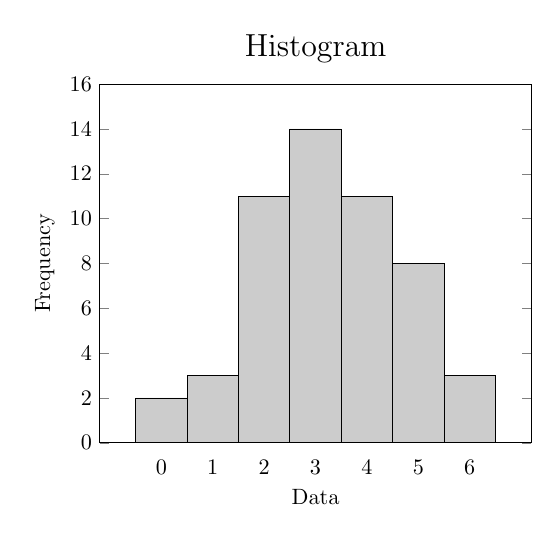
\begin{tikzpicture}[scale=0.8]
      \begin{axis}[
          title=\Large{Histogram},
          ymin=0, ymax=16,
          ytick={0, 2, ..., 16},
          xlabel=Data, ylabel=Frequency,
          ybar interval,
          grid=none,
          xtick style={draw=none},
        ]
        \addplot+[draw=black, style={fill=gray!40},mark=no] plot coordinates { (0, 2) (1, 3) (2, 11) (3, 14) (4, 11) (5, 8) (6, 3) (7, 0) };
      \end{axis}
    \end{tikzpicture}
  \end{center}

  The frequency polygon is a continuous line graph, the x-axis is the midpoint of
  each class, and the y-axis is the frequency of each class. To draw a frequency
  polygon, we plot each point, including the point before the first class and the
  point after the last class that uses $0$ as their frequency, and then connect
  the points with a continuous line.

  \begin{center}
    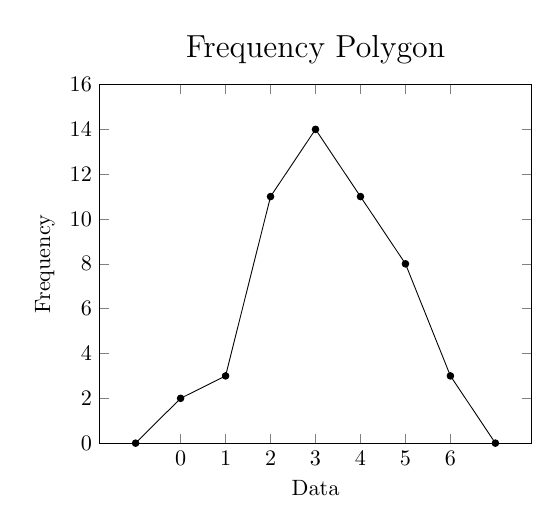
\begin{tikzpicture}[scale=0.8]
      \begin{axis}[
          title=\Large{Frequency Polygon},
          ymin=0, ymax=16,
          ytick={0, 2, ..., 16},
          xtick={0,1,...,6},
          xlabel=Data, ylabel=Frequency,
        ]
        \addplot[sharp plot, mark=*, mark size=1.5pt, mark options={solid, fill=black, draw=black}, draw=black]
        coordinates
          {(-1, 0) (0, 2) (1, 3) (2, 11) (3, 14) (4, 11) (5, 8) (6, 3) (7, 0)};
      \end{axis}
    \end{tikzpicture}
  \end{center}

  \begin{center}
    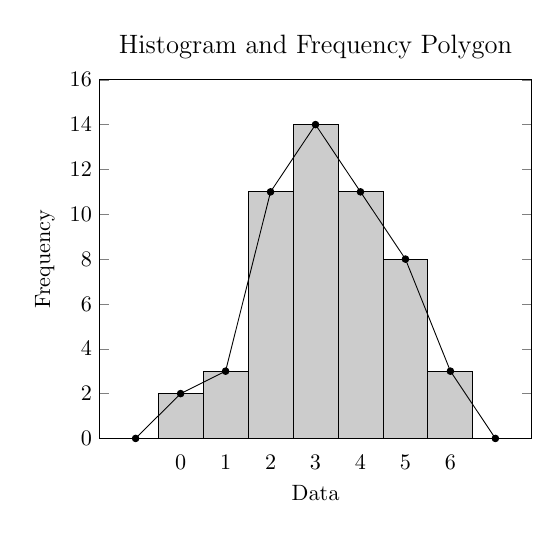
\begin{tikzpicture}[scale=0.8]
      \begin{axis}[
          title=\large{Histogram and Frequency Polygon},
          ymin=0, ymax=16,
          ytick={0, 2, ..., 16},
          xtick={0,1,...,6},
          ybar interval,
          grid=none,
          xtick style={draw=none},
          xlabel=Data, ylabel=Frequency,
        ]
        \addplot[draw=black, style={fill=gray!40},mark=no] plot coordinates { (0, 2) (1, 3) (2, 11) (3, 14) (4, 11) (5, 8) (6, 3) (7, 0) };
        \addplot[forget plot, sharp plot, mark=*, mark size=1.5pt, mark options={solid, fill=black, draw=black}, draw=black]
        coordinates
          {(-0.5, 0) (0.5, 2) (1.5, 3) (2.5, 11) (3.5, 14) (4.5, 11) (5.5, 8) (6.5, 3) (7.5, 0)};
      \end{axis}
    \end{tikzpicture}
  \end{center}

  \subsection{Practice 1}

  There are 105 students in a senior 3 art and commerce class. In a mock exam of
  UEC, their scores for Mathematics subject are as follows:
  \begin{flalign*}
    35 & \qquad 88 \qquad 67 \qquad 32 \qquad 38 \qquad 34 \qquad 45 \\
    78 & \qquad 54 \qquad 58 \qquad 69 \qquad 21 \qquad 90 \qquad 78 \\
    74 & \qquad 43 \qquad 42 \qquad 35 \qquad 57 \qquad 34 \qquad 77 \\
    89 & \qquad 66 \qquad 74 \qquad 71 \qquad 44 \qquad 56 \qquad 48 \\
    33 & \qquad 24 \qquad 73 \qquad 63 \qquad 51 \qquad 59 \qquad 49 \\
    34 & \qquad 55 \qquad 52 \qquad 75 \qquad 72 \qquad 62 \qquad 62 \\
    44 & \qquad 48 \qquad 73 \qquad 49 \qquad 57 \qquad 67 \qquad 80 \\
    70 & \qquad 66 \qquad 54 \qquad 32 \qquad 29 \qquad 35 \qquad 37 \\
    47 & \qquad 41 \qquad 51 \qquad 36 \qquad 46 \qquad 55 \qquad 53 \\
    60 & \qquad 53 \qquad 62 \qquad 39 \qquad 35 \qquad 48 \qquad 42 \\
    71 & \qquad 63 \qquad 70 \qquad 33 \qquad 45 \qquad 42 \qquad 44 \\
    61 & \qquad 59 \qquad 67 \qquad 30 \qquad 42 \qquad 43 \qquad 89 \\
    96 & \qquad 82 \qquad 47 \qquad 63 \qquad 54 \qquad 34 \qquad 45 \\
    45 & \qquad 87 \qquad 28 \qquad 34 \qquad 29 \qquad 77 \qquad 64 \\
    64 & \qquad 50 \qquad 48 \qquad 75 \qquad 33 \qquad 56 \qquad 84
  \end{flalign*}

  \begin{enumerate}[label=(\alph*)]
    \item Find the range of the data. \sol{}
          \begin{flalign*}
            \text{Max value}         & = 96      \\
            \text{Min value}         & = 21      \\
            \therefore\ \text{Range} & = 96 - 21 \\
                                     & = 75
          \end{flalign*}

    \item Group the data into 10 classes, draw a frequency distribution table, and find
          the upper and lower boundary and midpoint of each class. \sol{}
          \begin{flalign*}
            \text{Range}             & = 75            \\
            \text{Number of classes} & = 10            \\
            \text{Class width}       & = \frac{75}{10} \\
                                     & = 7.5           \\
                                     & \approx 8
          \end{flalign*}
          \begin{center}
            \begin{tabular}{|c|c|c|c|c|}
              \hline
              \text{Score} & \text{Lower} & \text{Upper} & \text{Mid} & \text{Freq.} \\
              \hline
              21 - 28      & 20.5         & 28.5         & 24.5       & 3            \\
              29 - 36      & 28.5         & 36.5         & 32.5       & 18           \\
              37 - 44      & 36.5         & 44.5         & 40.5       & 13           \\
              45 - 52      & 44.5         & 52.5         & 48.5       & 17           \\
              53 - 60      & 52.5         & 60.5         & 56.5       & 15           \\
              61 - 68      & 60.5         & 68.5         & 64.5       & 14           \\
              69 - 76      & 68.5         & 76.5         & 72.5       & 12           \\
              77 - 84      & 76.5         & 84.5         & 80.5       & 7            \\
              85 - 92      & 84.5         & 92.5         & 88.5       & 5            \\
              93 - 100     & 92.5         & 100.5        & 96.5       & 1            \\
              \hline
            \end{tabular}
          \end{center}
    \item Construct a histogram and frequency polygon. \sol{}
          \begin{center}
            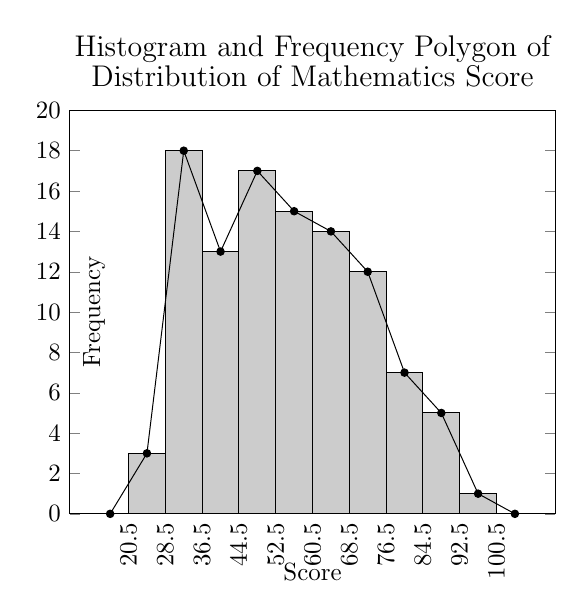
\begin{tikzpicture}[scale=0.9]
              \begin{axis}[
                  title style = {align = center},
                  title={\large{Histogram and Frequency Polygon of} \\ \large{Distribution of Mathematics Score}},
                  ymin=0, ymax=20,
                  ytick={0, 2, ..., 20},
                  xtick={20.5, 28.5, ..., 100.5},
                  grid=none,
                  xtick style={draw=none, fill=none, font=\footnotesize},
                  x tick label style = {rotate=90,anchor=east},
                  xlabel=Score, ylabel=Frequency,
                  xlabel style={at={(axis description cs:0.5, -0.1)}, anchor=north},
                  ylabel style={at={(axis description cs:0.05, 0.5)}, anchor=center},
                ]
                \addplot[ybar interval, draw=black, style={fill=gray!40},mark=no] plot coordinates { (20.5, 3) (28.5, 18) (36.5, 13) (44.5, 17) (52.5, 15) (60.5, 14) (68.5, 12) (76.5, 7) (84.5, 5) (92.5, 1) (100.5, 0) };
                \addplot[forget plot, sharp plot, mark=*, mark size=1.5pt, mark options={solid, fill=black, draw=black}, draw=black]
                coordinates
                  { (16.5, 0) (24.5, 3) (32.5, 18) (40.5, 13) (48.5, 17) (56.5, 15) (64.5, 14) (72.5, 12) (80.5, 7) (88.5, 5) (96.5, 1) (104.5, 0) };
              \end{axis}
            \end{tikzpicture}
          \end{center}
  \end{enumerate}

  \subsection*{Cumulative Frequency Distribution}

  Summing up the frequency of each class, we obtain the cumulative frequency
  distribution. Use the upper boundary of each class as the x-axis, and the
  cumulative frequency as the y-axis, we can draw the cumulative frequency
  distribution by plotting each point including the point before the first class
  that uses 0 as its frequency and connect them together. If we split the x-axis
  and the higest point of the curve into 100 equal parts, we get the percentage
  of the cumulative frequency distribution.

  \subsection{Practice 2}

  There are 155 students in a senior 3 art and commerce class, and the frequency
  distribution table of their average marks is shown below:

  \begin{center}
    \begin{tabular}{|c|c|}
      \hline
      \text{Average Mark} & \text{Frequency} \\
      \hline
      50 - 55             & 3                \\
      55 - 60             & 8                \\
      60 - 65             & 25               \\
      65 - 70             & 38               \\
      70 - 75             & 46               \\
      75 - 80             & 19               \\
      80 - 85             & 12               \\
      85 - 90             & 4                \\
      \hline
    \end{tabular}
  \end{center}

  \begin{enumerate}[label=(\alph*)]
    \item Make a cumulative frequency distribution table and draw a cumulative frequency
          polygon.

          \sol{}
          \begin{center}
            \begin{tabular}{|c|c|c|c|}
              \hline
              \text{Avg} & \text{Freq.} & \text{Lower Than} & \text{Cumm. Freq.} \\
              \hline
              50 - 55    & 3            & 55                & 3                  \\
              55 - 60    & 8            & 60                & 11                 \\
              60 - 65    & 25           & 65                & 36                 \\
              65 - 70    & 38           & 70                & 74                 \\
              70 - 75    & 46           & 75                & 120                \\
              75 - 80    & 19           & 80                & 139                \\
              80 - 85    & 12           & 85                & 151                \\
              85 - 90    & 4            & 90                & 155                \\
              \hline
            \end{tabular}
          \end{center}

          \begin{center}
            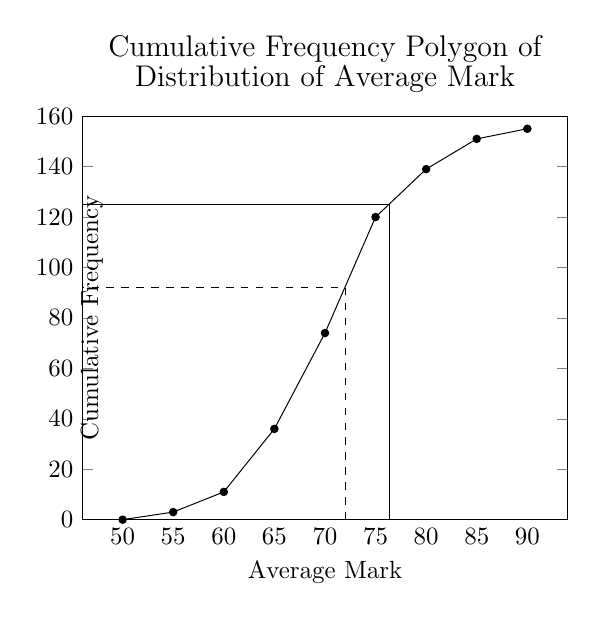
\begin{tikzpicture}[scale=0.9]
              \begin{axis}[
                  title style = {align = center},
                  title={\large{Cumulative Frequency Polygon of} \\ \large{Distribution of Average Mark}},
                  ymin=0, ymax=160,
                  ytick={0, 20, ..., 160},
                  xtick={50, 55, 60, ..., 90},
                  xtick style={draw=none, fill=none, font=\footnotesize},
                  xlabel=Average Mark, ylabel=Cumulative Frequency,
                  ylabel style={at={(axis description cs:0.02, 0.5)}, anchor=center},
                ]
                \addplot[forget plot, sharp plot, mark=*, mark size=1.5pt, mark options={solid, fill=black, draw=black}, draw=black]
                coordinates
                  { (50, 0) (55, 3) (60, 11) (65, 36) (70, 74) (75, 120) (80, 139) (85, 151) (90, 155) };
                \draw[dashed] (axis cs:72, 0) -- (axis cs:72, 92) -- (axis cs:0, 92);
                \draw (axis cs:0, 125) -- (axis cs:76.4, 125) -- (axis cs:76.4, 0);
              \end{axis}
            \end{tikzpicture}
          \end{center}

    \item If the average mark of a student is 72, find his rank in the class. \sol{}

          In the graph above, we can see that there are approximately 92 students who
          have an average mark lower than 72. Therefore, the rank of the student is $155
            - 92 = 63$.

    \item If the top $20\%$ of the class are to be awarded a certificate, find the
          minimum average mark required for the certificate. \sol{}
          \begin{flalign*}
            \text{Top $20\%$} & = 20\% \times 155 \\
                              & = 31
          \end{flalign*}
          Therefore, students with an average mark corresponding to cumulative frequency higher than 124 will be awarded a certificate.

          In the graph above, The minimum average mark required for the certificate is
          76.
  \end{enumerate}

  \subsection{Exercise 18.2}

  \begin{enumerate}
    \item A company performed an ability test on 100 job seekers and the results are
          shown in the following table:
          \begin{center}
            \begin{tabular}{|c|c|c|c|c|c|c|}
              \hline
              \text{Score}     & 8 & 7  & 6  & 5  & 4  & 3 \\
              \hline
              \text{Frequency} & 5 & 12 & 24 & 33 & 19 & 7 \\
              \hline
            \end{tabular}
          \end{center}
          Construct a hustogram and a frequency polygon for the data above.
          \sol{}
          \begin{center}
            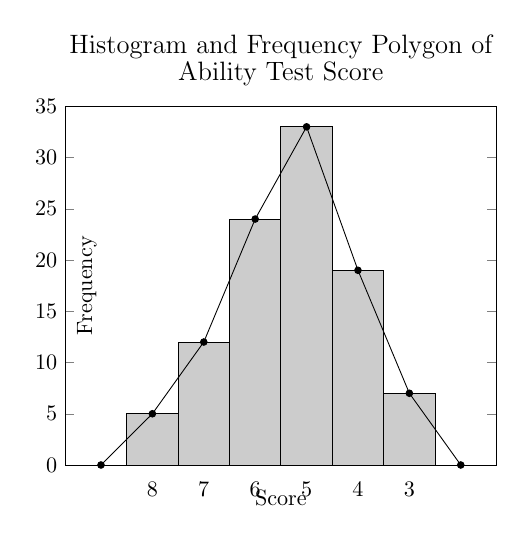
\begin{tikzpicture}[scale=0.8]
              \begin{axis}[
                  title style = {align = center},
                  title={\large{Histogram and Frequency Polygon of} \\ \large{Ability Test Score}},
                  ymin=0, ymax=35,
                  ytick={0, 5, ..., 35},
                  x dir=reverse,
                  ybar interval,
                  grid=none,
                  xtick style={draw=none},
                  xlabel=Score, ylabel=Frequency,
                  xlabel style={at={(axis description cs:0.5, -0.05)}, anchor=north},
                  ylabel style={at={(axis description cs:0.05, 0.5)}, anchor=center},
                ]
                \addplot[draw=black, style={fill=gray!40},mark=no] plot coordinates { (8, 5) (7, 12) (6, 24) (5, 33) (4, 19) (3, 7) (2, 0) };
                \addplot[forget plot, sharp plot, mark=*, mark size=1.5pt, mark options={solid, fill=black, draw=black}, draw=black]
                coordinates
                  {(8.5, 0) (7.5, 5) (6.5, 12) (5.5, 24) (4.5, 33) (3.5, 19) (2.5, 7) (1.5, 0)};
              \end{axis}
            \end{tikzpicture}
          \end{center}

    \item Take 120 ears of rice from a rice field, the length of each ear is measured (in
          $cm$) and the results are as following:
          \begin{flalign*}
            6.5 & \qquad 6.4 \qquad 6.7 \qquad 5.8 \qquad 5.9 \qquad 5.9 \\
            5.2 & \qquad 4.0 \qquad 5.4 \qquad 4.6 \qquad 5.8 \qquad 5.5 \\
            6.0 & \qquad 6.5 \qquad 5.1 \qquad 6.2 \qquad 5.4 \qquad 5.0 \\
            5.0 & \qquad 6.8 \qquad 6.0 \qquad 5.0 \qquad 5.7 \qquad 6.0 \\
            5.5 & \qquad 6.8 \qquad 6.0 \qquad 6.3 \qquad 5.5 \qquad 5.0 \\
            6.4 & \qquad 5.8 \qquad 5.9 \qquad 5.7 \qquad 6.8 \qquad 6.6 \\
            6.0 & \qquad 6.4 \qquad 5.7 \qquad 7.4 \qquad 6.0 \qquad 5.4 \\
            6.5 & \qquad 6.0 \qquad 6.8 \qquad 5.3 \qquad 6.4 \qquad 5.7 \\
            6.7 & \qquad 6.2 \qquad 5.6 \qquad 6.0 \qquad 6.7 \qquad 6.7 \\
            6.0 & \qquad 5.5 \qquad 6.2 \qquad 6.1 \qquad 5.3 \qquad 6.2 \\
            5.8 & \qquad 5.3 \qquad 7.0 \qquad 6.0 \qquad 6.0 \qquad 5.9 \\
            5.4 & \qquad 6.0 \qquad 5.2 \qquad 6.0 \qquad 6.3 \qquad 5.7 \\
            6.8 & \qquad 6.1 \qquad 4.5 \qquad 5.4 \qquad 6.3 \qquad 6.9 \\
            4.9 & \qquad 5.1 \qquad 5.6 \qquad 5.9 \qquad 6.1 \qquad 6.5 \\
            6.6 & \qquad 5.7 \qquad 5.8 \qquad 5.8 \qquad 6.2 \qquad 6.3 \\
            6.5 & \qquad 5.3 \qquad 5.9 \qquad 5.5 \qquad 5.8 \qquad 6.3 \\
            5.2 & \qquad 6.0 \qquad 7.0 \qquad 6.4 \qquad 5.8 \qquad 6.3 \\
            6.0 & \qquad 6.3 \qquad 5.6 \qquad 6.8 \qquad 6.6 \qquad 4.7 \\
            5.7 & \qquad 5.7 \qquad 5.6 \qquad 6.3 \qquad 6.0 \qquad 5.8 \\
            6.3 & \qquad 7.5 \qquad 6.2 \qquad 6.4 \qquad 7.0 \qquad 6.5
          \end{flalign*}

          \begin{enumerate}
            \item Find the range of the dataset. \sol{}
                  \begin{flalign*}
                    \text{Min value}         & = 4.0       \\
                    \text{Max value}         & = 7.5       \\
                    \therefore\ \text{Range} & = 7.5 - 4.0 \\
                                             & = 3.5
                  \end{flalign*}
            \item Group the data into 12 classes, make a frequency distribution table, find the
                  upper and lower boundaries and midpoint of each class, and calculate the
                  cumulative frequency. \sol{}
                  \begin{flalign*}
                    \text{Range}                   & = 3.5            \\
                    \text{Number of classes}       & = 12             \\
                    \therefore\ \text{Class width} & = \frac{3.5}{12} \\
                                                   & = \frac{3.5}{12} \\
                                                   & \approx 0.3
                  \end{flalign*}
                  \begin{center}
                    \begin{tabular}{|c|c|c|c|c|}
                      \hline
                      Weight    & Lower & Upper & Mid  & Freq. \\
                      \hline
                      4.0 - 4.2 & 3.95  & 4.25  & 4.10 & 1     \\
                      4.3 - 4.5 & 4.25  & 4.55  & 4.40 & 1     \\
                      4.6 - 4.8 & 4.55  & 4.85  & 4.70 & 2     \\
                      4.9 - 5.1 & 4.85  & 5.15  & 5.00 & 7     \\
                      5.2 - 5.4 & 5.15  & 5.45  & 5.30 & 12    \\
                      5.5 - 5.7 & 5.45  & 5.75  & 5.60 & 17    \\
                      5.8 - 6.0 & 5.75  & 6.05  & 5.90 & 31    \\
                      6.1 - 6.3 & 6.05  & 6.35  & 6.20 & 18    \\
                      6.4 - 6.6 & 6.35  & 6.65  & 6.50 & 15    \\
                      6.7 - 6.9 & 6.65  & 6.95  & 6.80 & 11    \\
                      7.0 - 7.2 & 6.95  & 7.25  & 7.10 & 3     \\
                      7.3 - 7.5 & 7.25  & 7.55  & 7.40 & 2     \\
                      \hline
                    \end{tabular}
                  \end{center}
                  \begin{center}
                    \begin{tabular}{|c|c|c|c|}
                      \hline
                      Weight    & Freq. & Lower Than & Cum. Freq. \\
                      \hline
                      4.0 - 4.3 & 1     & 4.3        & 1          \\
                      4.3 - 4.6 & 1     & 4.6        & 2          \\
                      4.6 - 4.9 & 2     & 4.9        & 4          \\
                      4.9 - 5.2 & 7     & 5.2        & 11         \\
                      5.2 - 5.5 & 12    & 5.5        & 23         \\
                      5.5 - 5.8 & 17    & 5.8        & 40         \\
                      5.8 - 6.1 & 31    & 6.1        & 71         \\
                      6.1 - 6.4 & 18    & 6.4        & 89         \\
                      6.4 - 6.7 & 15    & 6.7        & 104        \\
                      6.7 - 7.0 & 11    & 7.0        & 115        \\
                      7.0 - 7.3 & 3     & 7.3        & 118        \\
                      7.3 - 7.6 & 2     & 7.6        & 120        \\
                      \hline
                    \end{tabular}
                  \end{center}

            \item Construct a frequency polygon. \sol{}
                  \begin{center}
                    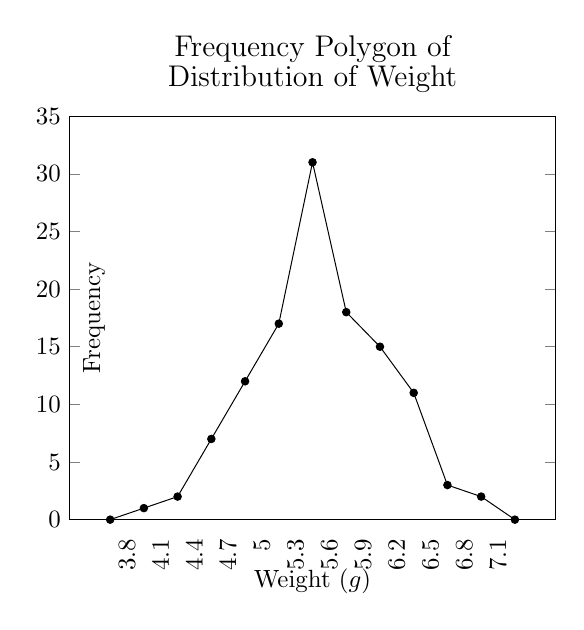
\begin{tikzpicture}[scale=0.9]
                      \begin{axis}[
                          title style = {align = center},
                          title={\large{Frequency Polygon of} \\ \large{Distribution of Weight}},
                          ymin=0, ymax=35,
                          ytick={0, 5, ..., 35},
                          ybar interval,
                          grid=none,
                          xtick style={draw=none, fill=none, font=\footnotesize},
                          x tick label style = {rotate=90,anchor=east},
                          xlabel=Weight ($g$), ylabel=Frequency,
                          xlabel style={at={(axis description cs:0.5, -0.1)}, anchor=north},
                          ylabel style={at={(axis description cs:0.05, 0.5)}, anchor=center},
                        ]
                        \addplot[forget plot, sharp plot, mark=*, mark size=1.5pt, mark options={solid, fill=black, draw=black}, draw=black]
                        coordinates
                          { (3.8, 0) (4.1, 1) (4.4, 2) (4.7, 7) (5.0, 12) (5.3, 17) (5.6, 31) (5.9, 18) (6.2, 15) (6.5, 11) (6.8, 3) (7.1, 2) (7.4, 0) };
                      \end{axis}
                    \end{tikzpicture}
                  \end{center}

            \item Construct a cumulative frequency polygon. \sol{}
                  \begin{center}
                    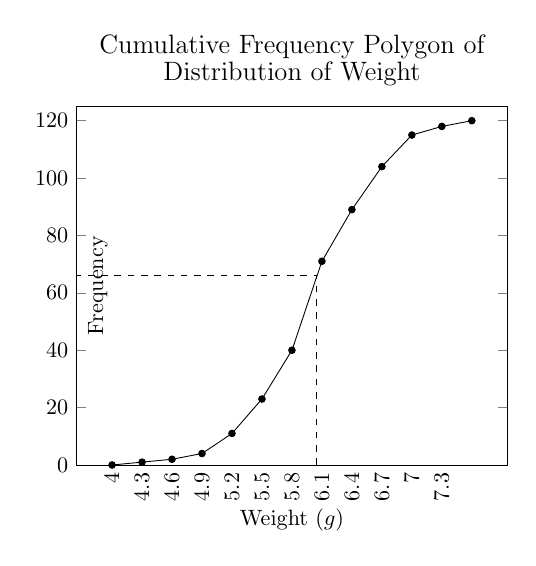
\begin{tikzpicture}[scale=0.8]
                      \begin{axis}[
                        title style = {align = center},
                        title={\large{Cumulative Frequency Polygon of} \\ \large{Distribution of Weight}},
                        ymin=0, ymax=125,
                        ytick={0, 20, ..., 120},
                        xtick={4.0, 4.3, 4.6, ..., 7.4},
                        xtick style={draw=none, fill=none, font=\footnotesize}, x tick label style =
                          {rotate=90,anchor=east}, xlabel=Weight ($g$), ylabel=Frequency, xlabel
                        style={at={(axis description cs:0.5, -0.1)}, anchor=north}, ylabel
                        style={at={(axis description cs:0.05, 0.5)}, anchor=center}, ] \addplot[forget
                          plot, sharp plot, mark=*, mark size=1.5pt, mark options={solid, fill=black,
                              draw=black}, draw=black] coordinates { (4.0, 0) (4.3, 1) (4.6, 2) (4.9, 4)
                            (5.2, 11) (5.5, 23) (5.8, 40) (6.1, 71) (6.4, 89) (6.7, 104) (7.0, 115) (7.3,
                            118) (7.6, 120) };
                        \draw [dashed] (axis cs: 6.05, 0) -- (axis cs: 6.05, 66) -- (axis cs: 0, 66);
                      \end{axis}
                    \end{tikzpicture}
                  \end{center}

            \item Find the percentage of the ears of rice whose length is greater than $6cm$.
                  \sol{}

                  In the diagram above, there are approximately $120 - 66 = 54$ ears of rice
                  whose length is greater than $6cm$, which is about $\frac{54}{120} \times 100\%
                    = 45\%$ of the total number of ears of rice.

          \end{enumerate}

    \item The table below shows the weight distribution of 90 babies (in $kg$):
          \begin{center}
            \begin{tabular}{|c|c|}
              \hline
              Weight    & Frequency \\
              \hline
              1.5 - 2.0 & 2         \\
              2.0 - 2.5 & 4         \\
              2.5 - 3.0 & 13        \\
              3.0 - 3.5 & 32        \\
              3.5 - 4.0 & 28        \\
              4.0 - 4.5 & 10        \\
              4.5 - 5.0 & 1         \\
              \hline
            \end{tabular}
          \end{center}
          \begin{enumerate}
            \item Make a cumulative frequency table. \sol{}
                  \begin{center}
                    \begin{tabular}{|c|c|c|c|}
                      \hline
                      Weight    & Freq. & Less than & Cum. Freq. \\
                      \hline
                      1.5 - 2.0 & 2     & 2.0       & 2          \\
                      2.0 - 2.5 & 4     & 2.5       & 6          \\
                      2.5 - 3.0 & 13    & 3.0       & 19         \\
                      3.0 - 3.5 & 32    & 3.5       & 51         \\
                      3.5 - 4.0 & 28    & 4.0       & 79         \\
                      4.0 - 4.5 & 10    & 4.5       & 89         \\
                      4.5 - 5.0 & 1     & 5.0       & 90         \\
                      \hline
                    \end{tabular}
                  \end{center}

            \item Construct a cumulative frequency polygon. \sol{}
                  \begin{center}
                    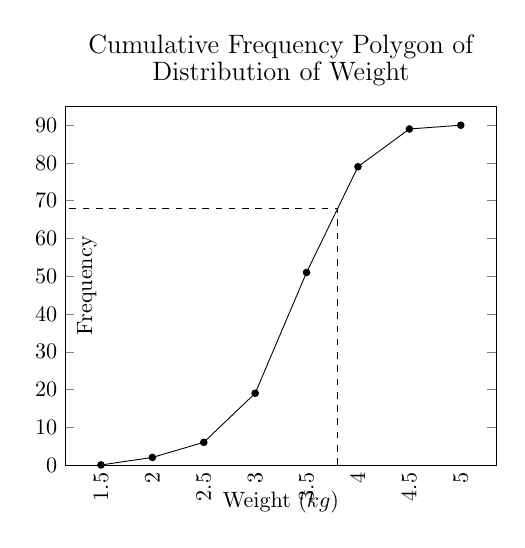
\begin{tikzpicture}[scale=0.8]
                      \begin{axis}[
                        title style = {align = center},
                        title={\large{Cumulative Frequency Polygon of} \\ \large{Distribution of Weight}},
                        ymin=0, ymax=95,
                        ytick={0, 10, ..., 90},
                        xtick={1.5, 2.0, 2.5, ..., 5.0},
                        xtick style={draw=none, fill=none, font=\footnotesize}, x tick label style =
                          {rotate=90,anchor=east}, xlabel=Weight ($kg$), ylabel=Frequency, xlabel
                        style={at={(axis description cs:0.5, -0.05)}, anchor=north}, ylabel
                        style={at={(axis description cs:0.05, 0.5)}, anchor=center}, ] \addplot[forget
                          plot, sharp plot, mark=*, mark size=1.5pt, mark options={solid, fill=black,
                              draw=black}, draw=black] coordinates { (1.5, 0) (2.0, 2) (2.5, 6) (3.0, 19)
                            (3.5, 51) (4.0, 79) (4.5, 89) (5.0, 90) };
                        \draw [dashed] (axis cs: 3.8, 0) -- (axis cs: 3.8, 68) -- (axis cs: 0, 68);
                      \end{axis}
                    \end{tikzpicture}
                  \end{center}

            \item Find the percentage of babies whose weight is greater than $3.8kg$. \sol{}

                  In the diagram above, there are approximately $90 - 68 = 22$ babies whose
                  weight is greater than $3.8kg$, which is about $\frac{22}{90} \times 100\% =
                    24.44\%$ of the total number of babies.
          \end{enumerate}

    \item The table below shows the average score distribution of 50 students in a class:
          \begin{center}
            \begin{tabular}{|c|c|}
              \hline
              Average Score & Frequency \\
              \hline
              50.0 - 59.9   & 4         \\
              60.0 - 69.9   & 9         \\
              70.0 - 79.9   & 23        \\
              80.0 - 89.9   & 12        \\
              90.0 - 99.9   & 2         \\
              \hline
            \end{tabular}
          \end{center}
          \begin{enumerate}
            \item Make a cumulative frequency table and draw a cumulative frequency polygon.
                  \sol{}
                  \begin{center}
                    \begin{tabular}{|c|c|c|c|}
                      \hline
                      Average Score & Freq. & Less than & Cum. Freq. \\
                      \hline
                      50.0 - 59.9   & 4     & 60        & 4          \\
                      60.0 - 69.9   & 9     & 70        & 13         \\
                      70.0 - 79.9   & 23    & 80        & 36         \\
                      80.0 - 89.9   & 12    & 90        & 48         \\
                      90.0 - 99.9   & 2     & 100       & 50         \\
                      \hline
                    \end{tabular}
                  \end{center}
                  \begin{center}
                    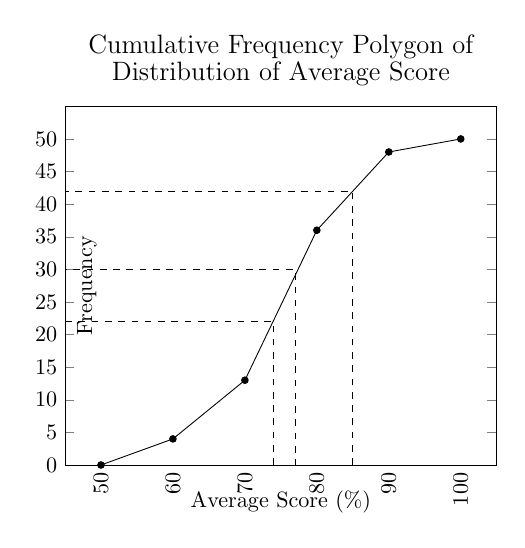
\begin{tikzpicture}[scale=0.8]
                      \begin{axis}[
                        title style = {align = center},
                        title={\large{Cumulative Frequency Polygon of} \\ \large{Distribution of Average Score}},
                        ymin=0, ymax=55,
                        ytick={0, 5, ..., 50},
                        xtick={50, 60, 70, 80, 90, 100},
                        xtick style={draw=none, fill=none, font=\footnotesize}, x tick label style =
                          {rotate=90,anchor=east}, xlabel=Average Score ($\%$), ylabel=Frequency, xlabel
                        style={at={(axis description cs:0.5, -0.05)}, anchor=north}, ylabel
                        style={at={(axis description cs:0.05, 0.5)}, anchor=center}, ] \addplot[forget
                          plot, sharp plot, mark=*, mark size=1.5pt, mark options={solid, fill=black,
                              draw=black}, draw=black] coordinates { (50, 0) (60, 4) (70, 13) (80, 36)
                            (90, 48) (100, 50) };
                        \draw [dashed] (axis cs: 74, 0) -- (axis cs: 74, 22) -- (axis cs: 0, 22);
                        \draw [dashed] (axis cs: 0, 30) -- (axis cs: 77, 30) -- (axis cs: 77, 0);
                        \draw [dashed] (axis cs: 85, 0) -- (axis cs: 85, 42) -- (axis cs: 0, 42);
                      \end{axis}
                    \end{tikzpicture}
                  \end{center}

            \item A student get an average score of $74$, find his rank in the class. \sol{}

                  In the diagram above, there are approximately $22$ students whose average score
                  is less than $74$, which means that the student is ranked $50 - 22 = 28$.

            \item Find the average score of the student who is ranked $20$. \sol{}

                  In the diagram above, the student who is ranked $20$ has an average score of
                  about $77$.

            \item Find the percentage of students whose average score is greater than $85$.
                  \sol{}

                  In the diagram above, there are approximately $50 - 42 = 8$ students whose
                  average score is greater than $85$, which is about $\frac{8}{50} \times 100\% =
                    16\%$ of the total number of students.
          \end{enumerate}

    \item The table below shows the score distribution of 1200 students in UEC accounting
          exam:
          \begin{center}
            \begin{tabular}{|c|c|}
              \hline
              Score   & Number of Students \\
              \hline
              10 - 19 & 20                 \\
              20 - 29 & 60                 \\
              30 - 39 & 95                 \\
              40 - 49 & 130                \\
              50 - 59 & 340                \\
              60 - 69 & 310                \\
              70 - 79 & 135                \\
              80 - 89 & 80                 \\
              90 - 99 & 30                 \\
              \hline
            \end{tabular}
          \end{center}
          Examinees are categorised into 4 groups based on their score: \textit{Excellent}, \textit{Good}, \textit{Pass}, and \textit{Fail}.
          \begin{enumerate}
            \item Make a cumulative frequency table and draw a cumulative frequency polygon.
                  \sol{}
                  \begin{center}
                    \begin{tabular}{|c|c|c|c|}
                      \hline
                      Score   & Freq. & Less than & Cum. Freq. \\
                      \hline
                      10 - 19 & 20    & 20        & 20         \\
                      20 - 29 & 60    & 80        & 80         \\
                      30 - 39 & 95    & 175       & 175        \\
                      40 - 49 & 130   & 305       & 305        \\
                      50 - 59 & 340   & 645       & 645        \\
                      60 - 69 & 310   & 955       & 955        \\
                      70 - 79 & 135   & 1090      & 1090       \\
                      80 - 89 & 80    & 1170      & 1170       \\
                      90 - 99 & 30    & 1200      & 1200       \\
                      \hline
                    \end{tabular}
                  \end{center}
                  \begin{center}
                    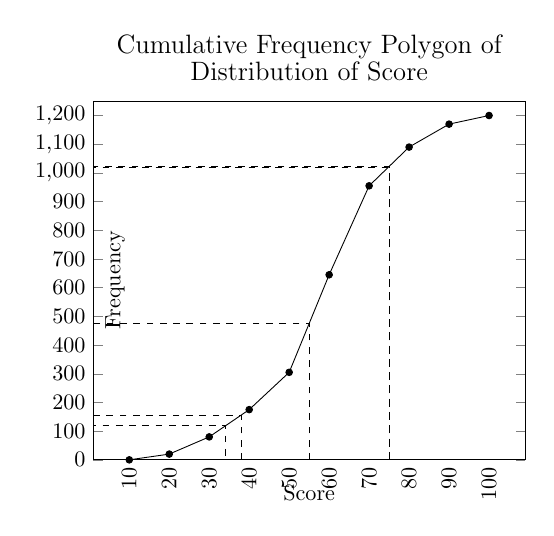
\begin{tikzpicture}[scale=0.8]
                      \begin{axis}[
                          title style = {align = center},
                          title={\large{Cumulative Frequency Polygon of} \\ \large{Distribution of Score}},
                          ymin=0, ymax=1250,
                          ytick={0, 100, ..., 1200},
                          xtick={10, 20, 30, 40, 50, 60, 70, 80, 90, 100},
                          xtick style={draw=none, fill=none, font=\footnotesize}, x tick label style =
                            {rotate=90,anchor=east}, xlabel=Score, ylabel=Frequency, xlabel style={at={(axis
                                  description cs:0.5, -0.05)}, anchor=north}, ylabel style={at={(axis
                                  description cs:0.05, 0.5)}, anchor=center}, ] \addplot[forget plot, sharp
                          plot, mark=*, mark size=1.5pt, mark options={solid, fill=black, draw=black},
                          draw=black] coordinates { (10, 0) (20, 20) (30, 80) (40, 175) (50, 305) (60,
                            645) (70, 955) (80, 1090) (90, 1170) (100, 1200) };
                        \draw [dashed] (axis cs: 38, 0) -- (axis cs: 38, 155) -- (axis cs: 0, 155);
                        \draw [dashed] (axis cs: 75, 0) -- (axis cs: 75, 1024) -- (axis cs: 0, 1024);
                        \draw [dashed] (axis cs: 55, 0) -- (axis cs: 55, 475) -- (axis cs: 0, 475);
                        \draw [dashed] (axis cs: 0, 120) -- (axis cs: 34, 120) -- (axis cs: 34, 0);
                        \draw [dashed] (axis cs: 0, 1020) -- (axis cs: 75, 1020) -- (axis cs: 75, 0);
                      \end{axis}
                    \end{tikzpicture}
                  \end{center}

            \item If the passing score is $38$, find the percentage of students who pass the
                  exam. \sol{}

                  In the diagram above, there are approximately $1200 - 155 = 1045$ students
                  whose score is greater or equal to $38$, which is about $\frac{1045}{1200}
                    \times 100\% = 86.67\%$ of the total number of students.

            \item Assume that the minimum score to be categorised as \textit{Excellent} and
                  \textit{Good} is $75$ and $55$ respectively, find the percentage of students
                  who are categorised as \textit{Excellent} and \textit{Good} respectively.
                  \sol{}

                  In the diagram above, there are approximately $1200 - 1024 = 176$ students
                  whose score is greater or equal to $75$, which is about $\frac{176}{1200}
                    \times 100\% = 14.67\%$ of the total number of students who are categorised as
                  \textit{Excellent}.

                  Also, there are approximately $1024 - 475 = 549$ students whose score is
                  greater or equal to $55$, which is about $\frac{549}{1200} \times 100\% =
                    45.75\%$ of the total number of students who are categorised as \textit{Good}.

            \item Find the passing mark if the percentage of students who pass the exam is
                  $90\%$. \sol{}

                  If the percentage of students who pass the exam is $90\%$, then the number of
                  students who pass the exam is $90\%$ of $1200$ students, which is $1080$
                  students. That means, there are $1200 - 1080 = 120$ students who fail the exam.

                  In the diagram above, the passing mark is about $34$ given that there are $120$
                  students who fail the exam.

            \item Find the minimum mark of a student who is categorised as \textit{Excellent} if
                  the percentage of students who are categorised as \textit{Excellent} is $15\%$.
                  \sol{}

                  If the percentage of students who are categorised as \textit{Excellent} is
                  $15\%$, then the number of students who are categorised as \textit{Excellent}
                  is $15\%$ of $1200$ students, which is $180$ students. That means, there are
                  $1200 - 180 = 1020$ students who are not categorised as \textit{Excellent}.

                  In the diagram above, the minimum mark of a student who is categorised as
                  \textit{Excellent} is about $75$ given that there are $1020$ students who are
                  not categorised as \textit{Excellent}.
          \end{enumerate}

  \end{enumerate}

  \section{Central Tendency}

  Central tendency is a measure of the central position of a distribution, or a
  single value that attempts to describe a set of data. The most common measures
  of central tendency are the mean, median, and mode.

  \subsection*{Mean}

  Mean is also known as arithmetic mean. For $n$ values $x_1, x_2, \ldots, x_n$,
  the mean is defined as \makeatletter \setbool{@fleqn}{false} \makeatother
  \begin{flalign*}
    \bar{x} & = \frac{x_1 + x_2 + \cdots + x_n}{n} \\
            & = \frac{\sum x_i}{n}
  \end{flalign*}
  \makeatletter
  \setbool{@fleqn}{true}
  \makeatother

  For data whose possible values are $x_1, x_2, \ldots, x_n$, and their
  respective frequencies are $f_1, f_2, \ldots, f_n$, the mean is defined as
  \makeatletter \setbool{@fleqn}{false} \makeatother
  \begin{flalign*}
    \bar{x} & = \frac{x_1f_1 + x_2f_2 + \cdots + x_nf_n}{f_1 + f_2 + \cdots + f_n} \\
            & = \frac{\sum f_i x_i}{\sum f_i}
  \end{flalign*}
  \makeatletter
  \setbool{@fleqn}{true}
  \makeatother

  For grouped data, we take the mean of each class as the representative value
  $x_i$ of the class.

  \subsubsection*{Weighted Mean}

  In some scenario, weighted mean is better than the mean to describe the data.

  When calculating the arithmetic mean, each value is given equal weight.
  However, in some cases, each value in a dataset may not be equally important.
  For example, the importance of the mark of a student for each subject is
  weighted according to the number of classes of the subject in a week. Hence,
  when calculating the average mark of the student, each mark must be multiplied
  by a value that represents the importance of the subject, and that value is
  called the weight. The weighted mean is defined as \makeatletter
  \setbool{@fleqn}{false} \makeatother
  \begin{flalign*}
    \bar{x} & = \frac{w_1x_1 + w_2x_2 + \cdots + w_n x_n}{w_1 + w_2 + \cdots + w_n} \\
            & = \frac{\sum w_i x_i}{\sum w_i}
  \end{flalign*}
  \makeatletter
  \setbool{@fleqn}{true}
  \makeatother
  where $x_i$ are the values and $w_i$ are the weights of $x_i$.

  \subsection{Practice 3}

  \begin{enumerate}
    \item Find the mean of 34, 50, 24, 32, 53, 30, 62, 27. \sol{}
          \begin{flalign*}
            \bar{x} & = \frac{30 + 50 + 24 + 32 + 53 + 30 + 62 + 27}{8} \\
                    & = \frac{312}{8}                                   \\
                    & = 39
          \end{flalign*}

    \item There are three workshop $A$, $B$, and $C$ in a factory. Workshop $A$ has 10
          workers, their wages are $\$35$ per day, workshop $B$ has 30 workers, their
          wages are $\$45$ per day, and workshop $C$ has 15 workers, their wages are
          $\$55$ per day. Find the mean of the wages of the workers in the factory.
          \sol{}

          Let the wages of workers be $x_1$, and the amount of workers be $f_1$.
          \begin{center}
            \begin{tabular}{|c|c|c|}
              \hline
              $x_1$ & $f_1$           & $x_1f_1$              \\
              \hline
              35    & 10              & 350                   \\
              45    & 30              & 1350                  \\
              55    & 15              & 825                   \\
              \hline
                    & $\sum f_i = 55$ & $\sum f_i x_i = 2525$ \\
              \hline
            \end{tabular}
          \end{center}
          $\therefore $ Average wages of workers in the factory is $\frac{2525}{55} = \$45.91$.

    \item A school appoints students to participate in a Math competition. During the
          competition, candidates must answer 25 questions within an hour. The table
          below shows the distribution of frequency of the number of questions that those
          candidates answer correctly:
          \begin{center}
            \begin{tabular}{|c|c|}
              \hline
              Answered Correctly & Frequency \\
              \hline
              1 - 5              & 3         \\
              6 - 10             & 12        \\
              11 - 15            & 7         \\
              16 - 20            & 8         \\
              21 - 25            & 5         \\
              \hline
            \end{tabular}
          \end{center}
          Complete the following table, and find the mean of the number of questions that those candidates answer correctly.
          \begin{center}
            \begin{tabular}{|c|c|c|c|}
              \hline
              Ans. Correctly & Freq. $f_i$ & Midpoint $x_i$ & $f_ix_i$ \\
              \hline
              1 - 5          &             &                &          \\
              6 - 10         &             &                &          \\
              11 - 15        &             &                &          \\
              16 - 20        &             &                &          \\
              21 - 25        &             &                &          \\
              \hline
            \end{tabular}
          \end{center}
          \sol{}
          \begin{center}
            \begin{tabular}{|c|c|c|c|}
              \hline
              Ans. Correctly & Freq. $f_i$     & Midpoint $x_i$       & $f_ix_i$ \\
              \hline
              1 - 5          & 3               & 3                    & 9        \\
              6 - 10         & 12              & 8                    & 96       \\
              11 - 15        & 7               & 13                   & 91       \\
              16 - 20        & 8               & 18                   & 144      \\
              21 - 25        & 5               & 23                   & 115      \\
              \hline
                             & $\sum f_i = 35$ & $\sum f_i x_i = 455$ &          \\
              \hline
            \end{tabular}
          \end{center}
          $\therefore $ The mean of the number of questions that those candidates answer correctly is $\frac{455}{35} = 13$.
  \end{enumerate}

  \subsection{Exercise 18.3a}

  \begin{enumerate}
    \item Take a sample of 20 from a batch of machine parts, their weight (in $g$) are as
          follows:
          \begin{flalign*}
            210 & \qquad 208 \qquad 200 \qquad 205 \qquad 202 \qquad 218 & \\
            206 & \qquad 214 \qquad 215 \qquad 207 \qquad 195 \qquad 207   \\
            218 & \qquad 192 \qquad 202 \qquad 216 \qquad 185 \qquad 227   \\
            187 & \qquad 215
          \end{flalign*}
          Find the mean weight of these machine parts.
          \sol{}
          \begin{flalign*}
            \bar{x} & = \frac{210 + 208 + 200 + \cdots + 215}{20} \\
                    & = \frac{4129}{20}                           \\
                    & = 206.45
          \end{flalign*}

    \item Given that the mean of a dataset 4, -3, 2, $k$, 5, 8 is 10, find the value of
          $k$. \sol{}
          \begin{flalign*}
            \frac{4 + (-3) + 2 + k + 5 + 8}{6} & = 10 \\
            16 + k                             & = 60 \\
            k                                  & = 44
          \end{flalign*}

    \item Given that the mean of $x_1$, $x_2$, $x_3$, $x_4$, $x_5$ is 40, and the mean of
          $y_1$, $y_2$, $y_3$ is 15. Find the mean after combining these two datasets.
          \sol{}
          \begin{flalign*}
            \frac{x_1 + \cdots + x_5}{5} & = 40                                 \\
            x_1 + \cdots + x_5           & = 200                                \\
            \\
            \frac{y_1 + y_2 + y_3}{3}    & = 15                                 \\
            y_1 + y_2 + y_3              & = 45                                 \\
            \\
            \bar{xy}                     & = \frac{x_1 + x_2 + \cdots + y_3}{8} \\
                                         & = \frac{245}{8}                      \\
                                         & = 30.63
          \end{flalign*}

    \item A school have 2 senior 3 classes: $A$ and $B$. In a Chinese language test, the
          average mark of 49 students in $A$ class in 72, while the average mark for 45
          students in class $B$ is 68. Find the average mark of all students in these two
          class combined. \sol{}
          \begin{flalign*}
            \bar{x} & = \frac{72 \times 49 + 68 \times 45}{49 + 45} \\
                    & = \frac{3528 + 3060}{94}                      \\
                    & = \frac{6588}{94}                             \\
                    & = 70.09
          \end{flalign*}

    \item Given that the mean for 8 values are 5. The mean increased by 1.4 after adding
          two values: $x$ and $3x$. Find the value of $x$. \sol{}
          \begin{flalign*}
            \frac{8 \times 5 + x + 3x}{8 + 2} & = 5 + 1.4 \\
            \frac{40 + 4x}{10}                & = 6.4     \\
            40 + 4x                           & = 64      \\
            4x                                & = 24      \\
            x                                 & = 6
          \end{flalign*}
    \item Throwing 6 coin at the same time and record the number of heads. After throwing
          100 times, we get the following frequency distribution table:
          \begin{center}
            \begin{tabular}{|c|c|}
              \hline
              Number of Heads & Frequency \\
              \hline
              0               & 2         \\
              1               & 10        \\
              2               & 24        \\
              3               & 35        \\
              4               & 22        \\
              5               & 6         \\
              6               & 1         \\
              \hline
            \end{tabular}
          \end{center}
          Find the mean of the number of heads for each throw.
          \sol{}

          Let the number of heads be $x_i$ and the frequency be $f_i$.
          \begin{center}
            \begin{tabular}{|c|c|c|}
              \hline
              $x_i$ & $f_i$            & $x_i f_i$           \\
              \hline
              0     & 2                & 0                   \\
              1     & 10               & 10                  \\
              2     & 24               & 48                  \\
              3     & 35               & 105                 \\
              4     & 22               & 88                  \\
              5     & 6                & 30                  \\
              6     & 1                & 6                   \\
              \hline
                    & $\sum f_i = 100$ & $\sum x_i f_i= 287$ \\
              \hline
            \end{tabular}
          \end{center}
          $\therefore$ The mean of the number of heads for each throw is $\frac{287}{100} = 2.87$.

    \item The table below shows the score distribution of 66 students in a Chinese
          language test:
          \begin{center}
            \begin{tabular}{|c|c|}
              \hline
              Score    & Frequency \\
              \hline
              31 - 40  & 6         \\
              41 - 50  & 12        \\
              51 - 60  & 15        \\
              61 - 70  & 15        \\
              71 - 80  & 8         \\
              81 - 90  & 6         \\
              91 - 100 & 4         \\
              \hline
            \end{tabular}
          \end{center}
          Find their mark in average.
          \begin{center}
            \begin{tabular}{|c|c|c|c|}
              \hline
              Score    & Mid $x_1$ & Freq. $f_1$     & $x_1f_1$             \\
              \hline
              31 - 40  & 35.5      & 6               & 213                  \\
              41 - 50  & 45.5      & 12              & 546                  \\
              51 - 60  & 55.5      & 15              & 832.5                \\
              61 - 70  & 65.5      & 15              & 982.5                \\
              71 - 80  & 75.5      & 8               & 604                  \\
              81 - 90  & 85.5      & 6               & 513                  \\
              91 - 100 & 95.5      & 4               & 382                  \\
              \hline
                       &           & $\sum f_1 = 66$ & $\sum x_1f_1 = 4073$ \\
              \hline
            \end{tabular}
          \end{center}
          $\therefore$ The mark in average is $\frac{4073}{66} = 61.71$.

    \item Below are the number of classes and marks for each subject of a junior student:
          \begin{center}
            \begin{tabular}{|c|c|c|}
              \hline
              Subject     & Number of Classes & Average Mark \\
              \hline
              Chinese     & 7                 & 75           \\
              Malay       & 7                 & 73           \\
              English     & 7                 & 65           \\
              Mathematics & 7                 & 82           \\
              Science     & 5                 & 86           \\
              History     & 3                 & 73           \\
              Geography   & 3                 & 87           \\
              \hline
            \end{tabular}
          \end{center}
          \begin{enumerate}
            \item Find his mark in average. \sol{}
                  \begin{flalign*}
                    \bar{x} & = \frac{75 + 73 + 65 + 82 + 86 + 73 + 87}{7} \\
                            & = \frac{541}{7}                              \\
                            & = 77.29
                  \end{flalign*}

            \item Use the number of classes as the weight to find his average mark. \sol{}
                  \begin{flalign*}
                    \bar{x} & = \frac{75 \times 7 + 73 \times 7 + \cdots + 87 \times 3}{7 + 7 + 7 + 7 + 5 + 3 + 3} & \\
                            & = \frac{525 + 511 + 455 + 574 + 430 + 219 + 261}{39}                                   \\
                            & = \frac{2975}{39}                                                                      \\
                            & = 76.28
                  \end{flalign*}
          \end{enumerate}
    \item The weight of 60 junior 2 students in a school are as follows:
          \begin{center}
            \begin{tabular}{|c|c|}
              \hline
              Weight (kg) & Frequency \\
              \hline
              54 - 56     & 10        \\
              57 - 59     & 20        \\
              60 - 62     & $x$       \\
              63 - 65     & 8         \\
              66 - 68     & 4         \\
              69 - 71     & $y$       \\
              \hline
            \end{tabular}
          \end{center}
          Given that the mean weight of these students is 60.1 kg, find the value of $x$ and $y$.
          \sol{}
          \begin{flalign*}
            \text{Total weight} & = 60.1 \times 60 = 3606
          \end{flalign*}
          \begin{center}
            \begin{tabular}{|c|c|c|c|}
              \hline
              Wght (kg) & M. $x_1$ & Freq. $f_1$     & $x_1f_1$             \\
              \hline
              54 - 56   & 55       & 10              & 550                  \\
              57 - 59   & 58       & 20              & 1160                 \\
              60 - 62   & 61       & $x$             & $61x$                \\
              63 - 65   & 64       & 8               & 512                  \\
              66 - 68   & 67       & 4               & 268                  \\
              69 - 71   & 70       & $y$             & $70y$                \\
              \hline
                        &          & $\sum f_1 = 60$ & $\sum x_1f_1 = 3606$ \\
              \hline
            \end{tabular}
          \end{center}
          \begin{numcases}{}
            10 + 20 + x + 8 + 4 + y = 60 \\
            550 + 1160 + 61x + 512 + 268 + 70y = 3606
          \end{numcases}
          \begin{flalign*}
            (1):             & \ 42 + x + y = 60  \\
                             & x + y = 18         \\
            (2):             & \ 61x + 70y = 1116 \\
            (1) \times 61:   & \ 61x + 61y = 1098 \\
            (2) - (1):       & \ 9y = 18          \\
                             & \ y = 2            \\
            \text{From }(1): & \ x = 16
          \end{flalign*}
  \end{enumerate}

  \subsection*{Median}

  The median is the middle value of a sorted dataset. The number of values must
  be equal for both side of the median.

  If the number of values is $n$, when $n$ is odd, the median is the number in
  $\frac{n+1}{2}$ position.\\ When $n$ is even, the median is the mean of the
  number in $\frac{n}{2}$ and $\frac{n}{2}+1$ position.

  For grouped data, we can make a cumulative frequency polygon, and the median is
  the value corresponding to $50\%$ of the percentage of the cumulative
  frequency.
  \begin{flalign*}
    \text{Let } & n \text{ be the number of values in the dataset, aka }\sum f_1, & \\
                & L_m \text{ be the lower boundaries of the group of the median,}   \\
                & C_m \text{ be the range of the group of the median,}              \\
                & f_m \text{ be the frequency of the group of the median,}          \\
                & F_m \text{ be the cum. frequency of the group of the median,}
  \end{flalign*}
  \begin{center}
    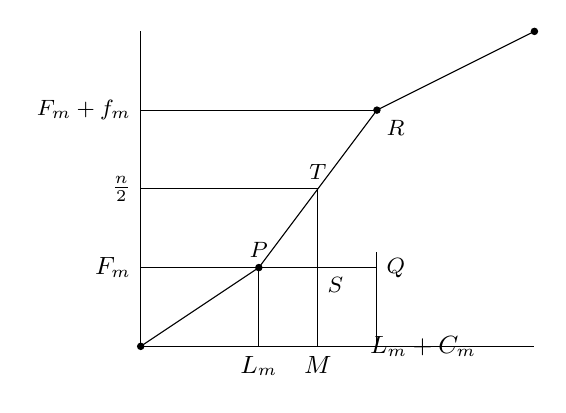
\begin{tikzpicture}
      \draw (0,0) -- (5,0);
      \draw (0,0) -- (0,4);
      \draw (0,0) -- (1.5, 1) -- (3, 3) -- (5, 4);
      \filldraw (0, 0) circle (0.04);
      \filldraw (1.5, 1) circle (0.04);
      \filldraw (3, 3) circle (0.04);
      \filldraw (5, 4) circle (0.04);
      \draw (0, 3) -- (3, 3);
      \draw (0, 2) -- (2.25, 2) -- (2.25, 0);
      \draw (1.5, 0) -- (1.5, 1) -- (0, 1);
      \draw (1.5, 1) -- (3, 1);
      \draw (3, 0) -- (3, 1.2);
      \draw (3, 1) node [right] {\footnotesize{${Q}$}};
      \draw (2.25, 1) node [below right] {\footnotesize{${S}$}};
      \draw (1.5, 1) node [above] {\footnotesize{${P}$}};
      \draw (2.25, 2) node [above] {\footnotesize{${T}$}};
      \draw (3, 3) node [below right] {\footnotesize{${R}$}};
      \draw (0, 3) node [left] {\footnotesize{$F_m + f_m$}};
      \draw (0, 2) node [left] {\small{$\frac{n}{2}$}};
      \draw (0, 1) node [left] {\small{$F_m$}};
      \draw (1.5, 0) node [below] {\small{$L_m$}};
      \draw (2.25, 0) node [below] {\small{$M$}};
      \draw (3, 0) node [below=8pt, right=-6pt] {\small{$L_m + C_m$}};
    \end{tikzpicture}
  \end{center}

  Diagram above shows a part of a cumulative frequency polygon, where $R$ is the
  point corresponding to the group containing the median, $P$ is the point
  corresponding to the group before the group containing the median, and $M$ is
  the median. Since $\Delta PQR \sim \Delta PST$,
  \begin{flalign*}
    \therefore \frac{PS}{PQ}             & = \frac{ST}{QR}                 \\
    \text{That is, } \frac{M - L_m}{C_m} & = \frac{\frac{n}{2} - F_m}{f_m}
  \end{flalign*}
  We get the following after simplifying the equation:
  \begin{cequation}
    M = L_m + \left(\frac{\frac{n}{2} - F_m}{f_m}\right)C_m
  \end{cequation}

  \subsection{Practice 4}

  \begin{enumerate}
    \item 10 workers in a factory made the same type of product in a day, the number of products made are as follows:
          \begin{flalign*}
            15 & \qquad 17 \qquad 14 \qquad 10 \qquad 15 \\
            19 & \qquad 17 \qquad 16 \qquad 14 \qquad 12
          \end{flalign*}
          Find the median of the number of products made by these 10 workers.
          \sol{}

          Sort the dataset:
          \begin{cequation}
            10 \quad 12 \quad 14 \quad 14 \quad 15 \quad 15 \quad 16 \quad 17 \quad 17 \quad 19
          \end{cequation}

          The median is the mean of the number in $\frac{10}{2} = 5$ and $\frac{10}{2}+1
            = 6$ position, which is $\frac{15 + 15}{2} = 15$.

    \item The table below shows the result of a right eye vision test for 49 students in
          a class:
          \begin{center}
            \begin{tabular}{|c|c|}
              \hline
              Vision & Number of Students \\
              \hline
              0.2    & 2                  \\
              0.3    & 3                  \\
              0.4    & 4                  \\
              0.5    & 3                  \\
              0.6    & 4                  \\
              0.8    & 9                  \\
              1.0    & 9                  \\
              1.2    & 10                 \\
              1.5    & 5                  \\
              \hline
            \end{tabular}
          \end{center}
          Find the median of the right eye vision of these students.
          \sol{}
          \begin{center}
            \begin{tabular}{|c|c|c|}
              \hline
              Vision & Number of Students & Cum. Frequency \\
              \hline
              0.2    & 2                  & 2              \\
              0.3    & 3                  & 5              \\
              0.4    & 4                  & 9              \\
              0.5    & 3                  & 12             \\
              0.6    & 4                  & 16             \\
              0.8    & 9                  & 25             \\\

              1.0    & 9                  & 34             \\
              1.2    & 10                 & 44             \\
              1.5    & 5                  & 49             \\
              \hline
            \end{tabular}
          \end{center}
          Since $n = 49$ is odd, the median is the number in the $\frac{49 + 1}{2} = 25$ position, which is $0.8$.

    \item The table below shows time distribution of 21 students browsing the Internet:
          \begin{center}
            \begin{tabular}{|c|c|}
              \hline
              Time (hours) & Number of Students \\
              \hline
              1.1 - 1.3    & 4                  \\
              1.4 - 1.6    & 3                  \\
              1.7 - 1.9    & 5                  \\
              2.0 - 2.2    & 4                  \\
              2.3 - 2.5    & 5                  \\
              \hline
            \end{tabular}
          \end{center}
          Find the median of the time distribution of these students.
          \sol{}
          \begin{center}
            \begin{tabular}{|c|c|c|}
              \hline
              Time      & Freq. & Cum. Freq. \\
              \hline
              1.1 - 1.3 & 4     & 4          \\
              1.4 - 1.6 & 3     & 7          \\
              1.7 - 1.9 & 5     & 12         \\
              2.0 - 2.2 & 4     & 16         \\
              2.3 - 2.5 & 5     & 21         \\
              \hline
            \end{tabular}
          \end{center}
          The median is the number in the $\frac{21}{2} = 10.5$ position, which is $1.7 - 1.9$.
          $C_m = 0.3$, $L_m = 1.65$, and $f_m = 5$, $F_m = 7$.
          \begin{flalign*}
            \therefore\ \textit{Mean} = 1.65 + \frac{10.5 - 7}{5} \times 0.3 = 1.86
          \end{flalign*}
  \end{enumerate}

  \subsection{Exercise 18.3b}

  \begin{enumerate}
    \item During a gymnastic competition, there are four judges scoring the performance
          of each contestant, and the median of these four scores are taken as the final
          score of the contestant. Given that the scores given by four judges are $9.5$,
          $9.4$, $9.8$, and $9.4$ respectively, find the final score of the contestant.
          \sol{}

          Sort the scores:
          \begin{cequation}
            9.4 \quad 9.4 \quad 9.5 \quad 9.8
          \end{cequation}
          The median is the mean of the number in $\frac{4}{2} = 2$ and $\frac{4}{2}+1 = 3$ position, which is $\frac{9.4 + 9.5}{2} = 9.45$.

    \item Following are the weight of 15 boys with same age:
          \begin{flalign*}
            36 & \qquad 35 \qquad 33 \qquad 37 \qquad 35 \\
            42 & \qquad 40 \qquad 38 \qquad 38 \qquad 39 \\
            40 & \qquad 41 \qquad 36 \qquad 38 \qquad 37
          \end{flalign*}
          \begin{enumerate}
            \item Find the median of these 15 boys. \sol{}

                  Sort the data:
                  \begin{flalign*}
                    33 & \quad 35 \quad 35 \quad 36 \quad 36 \quad 37 \quad 37 \quad 38 \quad 38 \quad 38 & \\
                    39 & \quad 40 \quad 41 \quad 42 \quad 43
                  \end{flalign*}
                  The median is the mean of the number in $\frac{15+1}{2} = 8$ position, which is $38$.

            \item Group the data using pattern $33 - 35$, $35 - 37$, $\ldots$, $41 - 43$. Then,
                  find the median. \sol{}
                  \begin{center}
                    \begin{tabular}{|c|c|c|}
                      \hline
                      Weight ($kg$) & Frequency & Cum. Frequency \\
                      \hline
                      33 - 35       & 1         & 1              \\
                      35 - 37       & 4         & 5              \\
                      37 - 39       & 5         & 10             \\
                      39 - 41       & 2         & 12             \\
                      41 - 43       & 2         & 14             \\
                      43 - 45       & 1         & 15             \\
                      \hline
                    \end{tabular}
                  \end{center}
                  The median is the number in the $\frac{15}{2} = 7.5$ position.
                  $C_m = 2$, $L_m = 37$, $f_m = 5$, and $F_m = 5$.
                  \begin{flalign*}
                    \therefore\ \textit{Median} = 37 + \frac{7.5 - 5}{5} \times 2 = 38
                  \end{flalign*}
          \end{enumerate}
    \item The table below shows the score distribution of a group of pupils in a minor
          test:
          \begin{center}
            \begin{tabular}{|c|c|}
              \hline
              Score & Number of Pupils \\
              \hline
              5     & 4                \\
              10    & 2                \\
              15    & 3                \\
              20    & $x$              \\
              25    & 4                \\
              \hline
            \end{tabular}
          \end{center}
          Assume that the median is 15, find the possibility value of $x$.
          \sol{}
          \begin{center}
            \begin{tabular}{|c|c|c|}
              \hline
              Score & Freq. & Cum. Freq. \\
              \hline
              5     & 4     & 4          \\
              10    & 2     & 6          \\
              15    & 3     & 9          \\
              20    & $x$   & 9 + x      \\
              25    & 4     & 13 + x     \\
              \hline
            \end{tabular}
          \end{center}
          \begin{flalign*}
            \frac{13 + x + 1}{2} & \leq 9     \\
            14 + x               & \leq 18    \\
            x                    & \leq 4     \\
            \therefore\ 0 \leq   & \ x \leq 4
          \end{flalign*}
          Therefore, the possibility values of $x$ are 0, 1, 2, 3, and 4.

    \item The following table shows the income of employees in a company:
          \begin{center}
            \begin{tabular}{|c|c|}
              \hline
              Income ($\$$) & Number of Employees \\
              \hline
              1000 - 2000   & 11                  \\
              2000 - 3000   & 17                  \\
              3000 - 4000   & 20                  \\
              4000 - 5000   & 10                  \\
              5000 - 6000   & 2                   \\
              \hline
            \end{tabular}
          \end{center}
          \begin{enumerate}
            \item Find the median of their income using cumulative frequency polygon. \sol{}
                  \begin{center}
                    \begin{tabular}{|c|c|c|}
                      \hline
                      Income ($\$$) & Freq. & Cum. Freq. \\
                      \hline
                      1000 - 2000   & 11    & 11         \\
                      2000 - 3000   & 17    & 28         \\
                      3000 - 4000   & 20    & 48         \\
                      4000 - 5000   & 10    & 58         \\
                      5000 - 6000   & 2     & 60         \\
                      \hline
                    \end{tabular}
                  \end{center}
                  The median is the number in $\frac{60}{2} = 30$ position.
                  \begin{center}
                    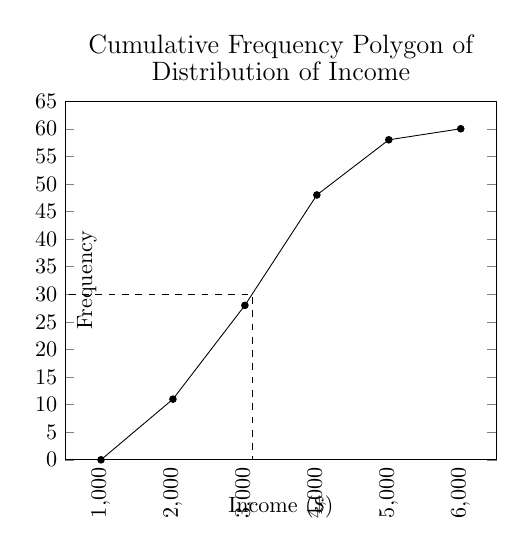
\begin{tikzpicture}[scale=0.8]
                      \begin{axis}[
                        title style = {align = center},
                        title={\large{Cumulative Frequency Polygon of} \\ \large{Distribution of Income}},
                        ymin=0, ymax=65,
                        ytick={0, 5, ..., 65},
                        xtick style={draw=none, fill=none, font=\footnotesize}, x tick label style =
                          {rotate=90,anchor=east}, xlabel=Income ($\$$), ylabel=Frequency, xlabel
                        style={at={(axis description cs:0.5, -0.08)}, anchor=north}, ylabel
                        style={at={(axis description cs:0.05, 0.5)}, anchor=center}, ] \addplot[forget
                          plot, sharp plot, mark=*, mark size=1.5pt, mark options={solid, fill=black,
                              draw=black}, draw=black] coordinates { (1000, 0) (2000, 11) (3000, 28) (4000, 48) (5000, 58) (6000, 60) };
                        \draw [dashed] (axis cs:0, 30) -- (axis cs:3100, 30) -- (axis cs:3100, 0);
                      \end{axis}
                    \end{tikzpicture}
                  \end{center}
                  Therefore, the median of their income is $\$3100$.

            \item Find the median of their income using formula and compare the result with (a).
                  \sol{}

                  The median is the number in the $\frac{60}{2} = 30$ position, which is $3000 -
                    4000$. $C_m = 1000$, $L_m = 3000$, and $f_m = 20$, $F_m = 28$.
                  \begin{cequation}
                    \therefore\ \textit{Median} = 3000 + \frac{30 - 28}{20} \times 1000 = 3100
                  \end{cequation}
                  Therefore, the median of their income is $\$3100$, which is the same as (a).
          \end{enumerate}

    \item The table below shows the distribution of height of 20 students:
          \begin{center}
            \begin{tabular}{|c|c|}
              \hline
              Height (cm) & Number of Students \\
              \hline
              120 - 130   & 3                  \\
              130 - 140   & 4                  \\
              140 - 150   & $x$                \\
              150 - 160   & 5                  \\
              160 - 170   & 6                  \\
              \hline
            \end{tabular}
          \end{center}
          Find:
          \begin{enumerate}
            \item The value of $x$. \sol{}
                  \begin{flalign*}
                    x + 3 + 4 + 5 + 6 & = 20      \\
                    x                 & = 20 - 18 \\
                                      & = 2
                  \end{flalign*}

            \item The median of their height. \sol{}
                  \begin{center}
                    \begin{tabular}{|c|c|c|}
                      \hline
                      Height $(cm)$ & Freq. & Cum. Freq. \\
                      \hline
                      120 - 130     & 3     & 3          \\
                      130 - 140     & 4     & 7          \\
                      140 - 150     & 2     & 9          \\
                      150 - 160     & 5     & 14         \\
                      160 - 170     & 6     & 20         \\
                      \hline
                    \end{tabular}
                  \end{center}
                  The median is the number in $\frac{20}{2} = 10$ position, which is $150 - 160$.
                  $C_m = 10$, $L_m = 150$, $f_m = 5$, and $F_m = 9$.
                  \begin{cequation}
                    \therefore\ \textit{Median} = 150 + \frac{10 - 9}{5} \times 10 = 152
                  \end{cequation}
                  Therefore, the median of their height is $152cm$.
          \end{enumerate}

    \item The table below shows the distribution of wages of workers in a factory:
          \begin{center}
            \begin{tabular}{|c|c|}
              \hline
              Wages $\$$ & Number of Workers \\
              \hline
              40 - 49    & 4                 \\
              50 - 59    & 14                \\
              60 - 69    & 5                 \\
              70 - 79    & $x$               \\
              80 - 89    & 2                 \\
              \hline
            \end{tabular}
          \end{center}
          Given that the median is $63.5$, find the value of $x$.
          \sol{}
          \begin{center}
            \begin{tabular}{|c|c|c|}
              \hline
              Wages $\$$ & Freq. & Cum. Freq. \\
              \hline
              40 - 49    & 4     & 4          \\
              50 - 59    & 14    & 18         \\
              60 - 69    & 5     & 23         \\
              70 - 79    & x     & 23 + x     \\
              80 - 89    & 2     & 25 + x     \\
              \hline
            \end{tabular}
          \end{center}

          $63.5$ is in between $60 - 69$, which is in the $\frac{25 + x}{2}$ position. $C_m = 10$, $L_m = 59.5$, $f_m = 5$, $F_m = 18$.
          \begin{flalign*}
            59.5 + \frac{\frac{25 + x}{2} - 18}{5} \times 10 & = 63.5 \\
            \frac{\frac{25 + x}{2} - 18}{5} \times 10        & = 4    \\
            \frac{\frac{25 + x}{2} - 18}{5}                  & = 0.4  \\
            \frac{25 + x}{2} - 18                            & = 2    \\
            \frac{25 + x}{2}                                 & = 20   \\
            25 + x                                           & = 40   \\
            x                                                & = 15
          \end{flalign*}
  \end{enumerate}

  \subsection*{Mode}

  In a set of data, the mode is the value that occurs most frequently. There can
  be more than one mode in a set of data. If all the values in a dataset occur
  with the same frequency, then there is no mode for the data.

  For grouped data, the mode is the class that has the highest frequency, and
  there can be more than one mode. Besides that, the mode can also be estimated
  using histogram. The method is as follows:

  \begin{center}
    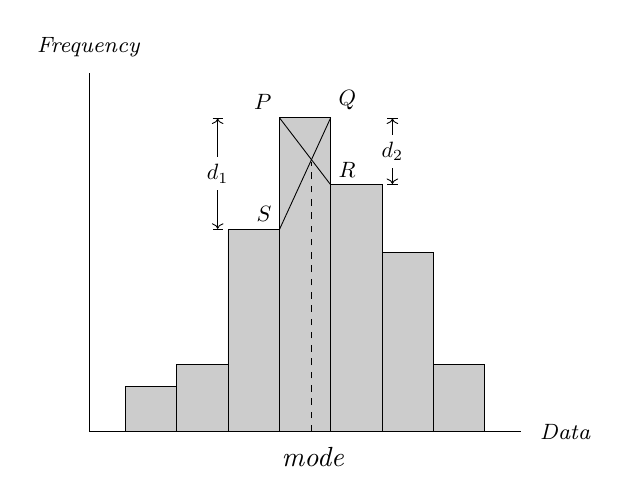
\begin{tikzpicture}[scale=0.8]
      \begin{axis}[
          ymin=0, ymax=16,
          ticks=none,
          ybar interval,
          grid=none,
          xtick style={draw=none},
          axis x line*=bottom,
          axis y line*=left,
        ]
        \addplot[draw=black, style={fill=gray!40},mark=no] plot coordinates { (0, 2) (1, 3) (2, 9) (3, 14) (4, 11) (5, 8) (6, 3) (7, 0) };
        \draw (axis cs:3, 9) -- (axis cs:4, 14);
        \draw (axis cs:3, 14) -- (axis cs:4, 11);
        \draw [dashed] (axis cs:3.63, 0) -- (axis cs: 3.63, 12);
        \node at (axis cs:3, 9) [above left] {$S$};
        \node at (axis cs:4, 14) [above right] {$Q$};
        \node at (axis cs:3, 14) [above left] {$P$};
        \node at (axis cs:4, 11) [above right] {$R$};
        \draw [|<->|] (axis cs:1.8, 9) -- (axis cs: 1.8, 14) node [midway, fill=white] {$d_1$};
        \draw [|<->|] (axis cs:5.2, 11) -- (axis cs: 5.2, 14) node [midway, fill=white] {$d_2$};
      \end{axis}
      \node at (3.55, -0.4) {$\textit{mode}$};
      \node at (7, 0) [right] {\footnotesize{\textit{Data}}};
      \node at (0, 5.8) [above] {\footnotesize{\textit{Frequency}}};
    \end{tikzpicture}
  \end{center}

  The diagram above shows a histogram of a set of data. The class corresponding
  to the highest rectangle is the mode of the data, and the mode is the x-value
  of the intersection point of $PR$ and $QS$.

  Unlike median, the formula of mode can be derived from similar triangles. Let:
  \begin{flalign*}
    L   & \text{ be the lower boundaries of the modal class}      \\
    C   & \text{ be the range of the modal class}                 \\
    d_1 & \text{ be the difference between the lower boundary of} \\
        & \text{ the modal class and the lower boundary of the}   \\
        & \text{ class immediately before the modal class}        \\
    d_2 & \text{ be the difference between the lower boundary of} \\
        & \text{ the modal class and the lower boundary of the}   \\
        & \text{ class immediately after the modal class}
  \end{flalign*}
  then
  \begin{cequation}
    \textit{mode} = L + \left(\frac{d_1}{d_1 + d_2}\right)C
  \end{cequation}

  \subsection{Practice 5}

  The following table shows the distribution of the score of 36 students in a
  Mathematics exam:
  \begin{center}
    \begin{tabular}{|c|c|}
      \hline
      Score   & Number of Students \\
      \hline
      20 - 29 & 2                  \\
      30 - 39 & 6                  \\
      40 - 49 & 10                 \\
      50 - 59 & 12                 \\
      60 - 69 & 3                  \\
      70 - 79 & 2                  \\
      80 - 89 & 1                  \\
      \hline
    \end{tabular}
  \end{center}
  \begin{enumerate}[label=(\alph*)]
    \item Find the modal class. \sol{}

          The modal class is $50 - 59$, which has the highest frequency of 12.

    \item Find the mode of score of the students using histogram. \sol{}
          \begin{center}
            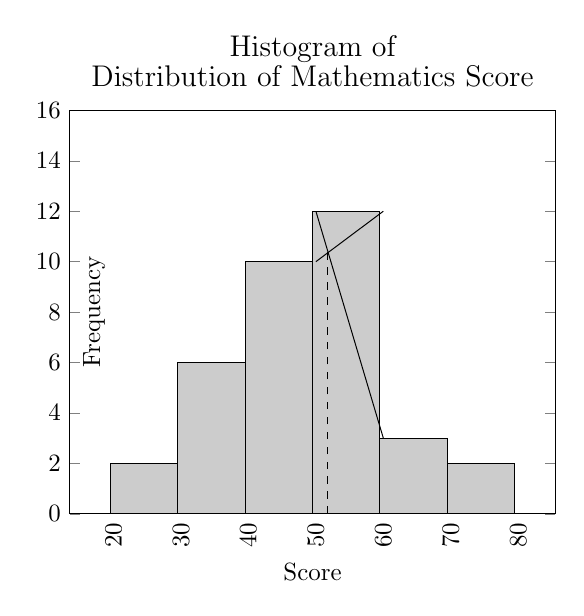
\begin{tikzpicture}[scale=0.9]
              \begin{axis}[
                  title style = {align = center},
                  title={\large{Histogram of} \\ \large{Distribution of Mathematics Score}},
                  ymin=0, ymax=16,
                  ytick={0, 2, ..., 16},
                  grid=none,
                  xtick style={draw=none, fill=none, font=\footnotesize},
                  x tick label style = {rotate=90,anchor=east},
                  xlabel=Score, ylabel=Frequency,
                  xlabel style={at={(axis description cs:0.5, -0.1)}, anchor=north},
                  ylabel style={at={(axis description cs:0.05, 0.5)}, anchor=center},
                ]
                \addplot[ybar interval, draw=black, style={fill=gray!40},mark=no] plot coordinates { (19.5, 2) (29.5, 6) (39.5, 10) (49.5, 12) (59.5, 3) (69.5, 2) (79.5, 1) };
                \draw (axis cs:50, 10) -- (axis cs:60, 12);
                \draw (axis cs:50, 12) -- (axis cs:60, 3);
                \draw [dashed] (axis cs:51.7, 0) -- (axis cs: 51.7, 10.5);
              \end{axis}
            \end{tikzpicture}
          \end{center}

          The mode of score of the students is approximately $51.5$.

    \item Find the mode of score of the students using formula. \sol{}

          $L = 49.5$, $C = 10$, $d_1 = 12 - 10 = 2$, $d_2 = 12 - 3 = 9$.
          \begin{flalign*}
            \therefore\ \textit{Mode} = 49.5 + \left(\frac{2}{2 + 9}\right)10 = 51.32
          \end{flalign*}

  \end{enumerate}

  \subsection*{Comparing mean, median and mode}

  Generally, the mean, median and mode of a set of data are all dirrent, and they
  are used to describe the data in different ways.

  \subsection{Exercise 18.3c}

  \begin{enumerate}
    \item Find the mode of the following data:
          \begin{enumerate}
            \item $3 \quad 4 \quad 3 \quad 2 \quad 4 \quad 5 \quad 5 \quad 5 \quad 4 \quad 4$
                  \sol{}

                  The mode is $4$, which has the highest frequency of 4.

            \item $7 \quad 6 \quad 8 \quad 8 \quad 5 \quad 6 \quad 6 \quad 9 \quad 8 \quad 5$
                  \sol{}

                  The mode is $6$ and $8$, which has the highest frequency of 3.

            \item $1.0 \quad 1.1 \quad 1.0 \quad 0.9 \quad 0.8 \quad 1.2 \quad 1.0 \quad 0.9 \quad 1.1 \quad$\\
                  $1.0$
                  \sol{}

                  The mode is $1.0$, which has the highest frequency of 4.
          \end{enumerate}
    \item In the sport competition of a high school, the scores of 17 athletes
          participating in men's high jump are as follows:
          \begin{center}
            \begin{tabular}{|c|c|}
              \hline
              Scores ($m$) & Number of Athletes \\ \hline
              1.50         & 2                  \\
              1.60         & 3                  \\
              1.65         & 2                  \\
              1.70         & 3                  \\
              1.75         & 4                  \\
              1.80         & 1                  \\
              1.85         & 1                  \\
              1.90         & 1                  \\
              \hline
            \end{tabular}
          \end{center}
          Find the mean, median and mode of their scores.
          \sol{}
          \begin{flalign*}
            \textit{Mean} & = \frac{1.50 \times 2 + 1.60 \times 3 + \cdots + 1.90 \times 1}{17} & \\
                          & = \frac{3 + 4.8 + 3.3 + 5.1 + 7 + 1.8 + 1.85 + 1.9}{17}               \\
                          & = \frac{28.75}{17}                                                    \\
                          & = 1.69m
          \end{flalign*}
          \begin{center}
            \begin{tabular}{|c|c|c|}
              \hline
              Scores ($m$) & No. of Athletes & Cum. Frequency \\ \hline
              1.50         & 2               & 2              \\
              1.60         & 3               & 5              \\
              1.65         & 2               & 7              \\
              1.70         & 3               & 10             \\
              1.75         & 4               & 14             \\
              1.80         & 1               & 15             \\
              1.85         & 1               & 16             \\
              1.90         & 1               & 17             \\
              \hline
            \end{tabular}
          \end{center}
          The median is the number at $\frac{17 + 1}{2} = 9$th position, which is $1.70m$.

          The mode is $1.75m$, which has the highest frequency of 4.

    \item In a Mathematics competition, the scores and the number of students who
          obtained the scores are as follows:
          \begin{center}
            \begin{tabular}{|c|c|}
              \hline
              Scores ($\%$) & Number of Students \\ \hline
              10 - 19       & 20                 \\
              20 - 29       & 60                 \\
              30 - 39       & 80                 \\
              40 - 49       & 40                 \\
              50 - 59       & 10                 \\
              \hline
            \end{tabular}
          \end{center}
          Find the modal class and the mode.
          \sol{}

          The modal clsas is $30 - 39$, which has the highest frequency of 80.

          $L = 29.5$, $C = 10$, $d_1 = 80 - 60 = 20$, $d_2 = 80 - 40 = 40$.
          \begin{flalign*}
            \therefore\ \textit{Mode} = 29.5 + \left(\frac{20}{20 + 40}\right)10 = 32.83
          \end{flalign*}

    \item Given that the mean of a dataset 3, 5, 8, 6, 8, 10, 5, 3, $x$, $y$ is 6,
          \begin{enumerate}
            \item Prove that $x+y = 12$ \prooff{}
                  \begin{flalign*}
                    \frac{3 + 5 + 8 + 6 + 8 + 10 + 5 + 3 + x + y}{10} & = 6  \\
                    48 + x + y                                        & = 60 \\
                    x + y                                             & = 12
                  \end{flalign*}
            \item With that, if
                  \begin{enumerate}
                    \item $x = y$
                    \item $x < y$
                  \end{enumerate}
                  Find the mode of the dataset.
          \end{enumerate}
    \item The mean of a set of data 13, 5, 5, $n$, 5, 10, 10, 11, 9, $n^2$ is $7.4$,
          \begin{enumerate}
            \item Find the possible values of $n$.
            \item With that, If
                  \begin{enumerate}
                    \item $n > 0$
                    \item $n < 0$
                  \end{enumerate}
                  Find the meadian of the dataset.
          \end{enumerate}
    \item The following table shows the distribution of scores of a group of students in
          a competition:
          \begin{center}
            \begin{tabular}{|c|c|}
              \hline
              Scores & Number of Students \\ \hline
              0      & 3                  \\
              1      & x                  \\
              2      & 4                  \\
              3      & 6                  \\
              4      & 2                  \\
              \hline
            \end{tabular}
          \end{center}
          \begin{enumerate}
            \item Assume that the mode is 1, find the minimum value of $x$.
            \item Assume that the median is 2, find the maximum value of $x$.
            \item Assume that the mean is $1.95$, find the value of $x$.
          \end{enumerate}
    \item Given thet the mode, median and mean of 5 positive integers are 9, 8, and $7.6$
          respectively, find these 5 numbers.
    \item The following table shows the amount of sales of a brand of shoes in a month:
          \begin{center}
            \begin{tabular}{|c|c|}
              \hline
              Shoes Number & Amount of Sales \\ \hline
              5            & 4               \\
              6            & 10              \\
              7            & 11              \\
              8            & 18              \\
              9            & 2               \\
              \hline
            \end{tabular}
          \end{center}
          \begin{enumerate}
            \item Find the mean, median, and mode.
            \item Which of the following central tendency represents the data best? Why?
          \end{enumerate}
    \item In between 54 examinees in an exam, 15 of them come from cities, 39 of them
          come from suburbs. Below are the frequency distribution table of their scores:
          \begin{center}
            \begin{tabular}{|c|c|c|}
              \hline
              Scores   & City & Suburb \\ \hline
              12 - 23  & 0    & 1      \\
              23 - 34  & 0    & 0      \\
              34 - 45  & 0    & 5      \\
              45 - 56  & 1    & 6      \\
              56 - 67  & 3    & 5      \\
              67 - 78  & 4    & 13     \\
              78 - 89  & 6    & 4      \\
              89 - 100 & 1    & 5      \\
              \hline
            \end{tabular}
          \end{center}
          \begin{enumerate}
            \item Find the mean, median, and mode of the scores of the examinees from cities and
                  suburbs respectively.
            \item Find the mean, median, and mode of the scores of all the examinees.
          \end{enumerate}
    \item The following table shows the distribution of scores of a group of students in
          a Chinese language test:
          \begin{center}
            \begin{tabular}{|c|c|}
              \hline
              Scores $x$       & Number of Students \\ \hline
              $40 < x \leq 50$ & 12                 \\
              $50 < x \leq 60$ & 30                 \\
              $60 < x \leq 70$ & 35                 \\
              $70 < x \leq 80$ & 25                 \\
              $80 < x \leq 90$ & 10                 \\
              $9 < x \leq 100$ & 3                  \\
              \hline
            \end{tabular}
          \end{center}
          Find:
          \begin{enumerate}
            \item Mean.
            \item Modal class and mode.
            \item Median.
          \end{enumerate}
  \end{enumerate}

  \section{Measures of Dispersion}

  The measures of dispersion can be used to describe the spread of the data.

  When we're describing a set of data, if we only use the mean, the information
  provided by the dataset is not enough. For example, given the mean, median, and
  mode of the average marks of four students in a Mathematics test are all 70
  marks, we can't tell the difference between the four students. Their marks
  might be similar (e.g. 68, 72, 70, 70) or they might be very different (e.g.
  100, 40, 70, 70). The latter case is obviously more spread out than the former
  case.

  The most common measures of dispersion are range, interquartile range, quartile
  deviation, standard deviation, mean deviation, variance, and standard
  deviation.

  \subsubsection*{Range}

  The range of a set of data is the difference between the largest and the
  smallest value in the dataset.

  For grouped data, the range is the difference between the upper limit of the
  highest class and the lower limit of the lowest class.

  \subsection*{Quartile, Interquartile Range, and Quartile Deviation}

  Quartiles are three value $Q_1$, $Q_2$, and $Q_3$ that divide a dataset into
  four equal parts. $Q_2$ is the median of the dataset. $Q_1$ and $Q_3$ are the
  medians of the two halves of the dataset, called the lower quartile and the
  upper quartile respectively.

  Assume that the number of data in a sorted dataset is $n$. If $n$ is odd, then

  When $n$ is even, split the dataset into two halves, with $n/2$ data in each
  half.

  When $n$ is odd, split the data into two halves after removing the median, with
  $(n-1)/2$ data in each half.

  The median of the lower half is $Q_1$ and the median of the upper half is
  $Q_3$.

  For grouped data, we can make a cumulative frequency polygon. In the percentage
  of the polygon,

  $25\%$ of the data is below $Q_1$.

  $50\%$ of the data is below $Q_2$.

  $75\%$ of the data is below $Q_3$.

  Using the same method of deriving the formula for median, we can derive the
  formula for upper and lower quartiles. Let
  \begin{flalign*}
    n   & \text{ be the number of data in the dataset, aka } \sum f_i \\
    L_k & \text{ be the lower boundaries of the class of } Q_k        \\
    C_k & \text{ be the class range of the class of } Q_k             \\
    f_k & \text{ be the frequency of the class of } Q_k               \\
    F_k & \text{ be the cumulative frequency of the class of } Q_k    \\
  \end{flalign*}
  then
  \begin{cequation}
    Q_1 = L_1 + \left(\frac{\frac{n}{4} - F_1}{f_1}\right)C_1
  \end{cequation}
  \begin{cequation}
    Q_2 = L_2 + \left(\frac{\frac{3n}{4} - F_2}{f_2}\right)C_2
  \end{cequation}

  The difference between the upper and lower quartiles is called the
  interquartile range. That is,
  \begin{cequation}
    \textit{Interquartile range} = Q_3 - Q_1
  \end{cequation}

  The quartile deviation is the interquartile range divided by 2, written as
  $Q.D.$, that is,
  \begin{cequation}
    \textit{Q.D.} = \frac{Q_3 - Q_1}{2}
  \end{cequation}

  Since the interquartile range and the quartile deviation are not affected by
  the outliers, they are more robust than the range, and are more suitable for
  representing the spread of the data.

  \subsection{Practice 6}

  \begin{enumerate}
    \item Find the range, quartiles and interquartile range of the following data:
          \begin{enumerate}
            \item 4 \quad 8 \quad 7 \quad 3 \quad 3 \quad 9 \quad 6 \quad 5 \quad 1 \quad 1 \quad 2
            \item 7 \quad 6 \quad 8 \quad 8 \quad 5 \quad 6 \quad 1 \quad 9 \quad 8
            \item 1.0 \quad 1.1 \quad 1.5 \quad 0.7 \quad 0.8 \quad 1.2 \quad 1.4\ \quad 0.9 \quad 1.6 \quad 1.3
            \item 3 \quad 4 \quad 7 \quad 2 \quad 4 \quad 6 \quad 5 \quad 8
          \end{enumerate}
    \item The table below shows the cumulative frequency distribution table of the
          heights of 60 students:
          \begin{center}
            \begin{tabular}{|c|c|}
              \hline
              Height ($cm$) & Cumulative Frequency \\
              \hline
              150-155       & 3                    \\
              155-160       & 10                   \\
              160-165       & 22                   \\
              165-170       & 37                   \\
              170-175       & 51                   \\
              175-180       & 58                   \\
              180-185       & 60                   \\
              \hline
            \end{tabular}
          \end{center}
          \begin{enumerate}
            \item Find the interquartile range of the heights of the students from the cumulative
                  frequency polygon.
            \item Find the interquartile range of the heights of the students using formula.
          \end{enumerate}
  \end{enumerate}

  \subsection{Exercise 18.4a}

  \begin{enumerate}
    \item Following are the sales of televisions of a shop in 11 days:
          \begin{flalign*}
            4 \quad 9 \quad 0 \quad 1 \quad 3 \quad 4 \quad 2 \quad 5 \quad 7 \quad 2 \quad 3
          \end{flalign*}
          Find:
          \begin{enumerate}
            \item The range.
            \item The quartiles and interquartile range.
          \end{enumerate}
    \item Given a set of data: 1.2, 1.0, 1.1, 1.3, 1.5, 1.7, 1.2, 1.0. Find:
          \begin{enumerate}
            \item The range.
            \item The quartiles and interquartile deviation.
          \end{enumerate}
    \item The distribution of scores of Mathematics test of 100 senior 1 students from a
          high school are as follows:
          \begin{center}
            \begin{tabular}{|c|c|}
              \hline
              Scores   & Number of Students \\
              \hline
              30 - 40  & 3                  \\
              40 - 50  & 4                  \\
              50 - 60  & 13                 \\
              60 - 70  & 22                 \\
              70 - 80  & 30                 \\
              80 - 90  & 23                 \\
              90 - 100 & 5                  \\
              \hline
            \end{tabular}
          \end{center}
          Find the interquartile deviation of the scores.
  \end{enumerate}

  \subsubsection*{Mean Deviation}

  Let the mean of a set of data $x_1$, $x_2$, $\ldots$, $x_n$ be $\bar{x}$, $|x_i
    - \bar{x}|$ is the difference between the $i$th data and the mean, the mean of
  these $n$ differences are called the mean deviation, and can be used to
  calculate the measure of dispersion of the data. That is,
  \begin{cequation}
    \textit{Mean Deviation} = \frac{\sum |x_i - \bar{x}|}{n}
  \end{cequation}

  If the possible value given data are $x_1$, $x_2$, $\ldots$, $x_n$, their
  frequencies are $f_1$, $f_2$, $\ldots$, $f_n$, respectively, then the mean
  deviation can be calculated as follows:
  \begin{cequation}
    \textit{Mean Deviation} = \frac{\sum |x_i - \bar{x}|f_i}{\sum f_i}
  \end{cequation}

  For grouped data, we take the midpoints of the classes as the representative
  value $x_i$.

  \subsection{Practice 7}

  Complete the following table, and find the mean and mean deviation of the data.
  \begin{center}
    \begin{tabular}{|c|c|c|c|c|c|}
      \hline
      Lim.    & Freq. $f_i$ & Mid. $x_i$ & $f_ix_i$ & $|x_i - \bar{x}|$ & $|x_i - \bar{x}|f_i$ \\
      \hline
      50 - 54 & 2           &            &          &                   &                      \\
      55 - 59 & 3           &            &          &                   &                      \\
      60 - 64 & 6           &            &          &                   &                      \\
      65 - 69 & 9           &            &          &                   &                      \\
      \hline
    \end{tabular}
  \end{center}

  \subsection{Exercise 18.4b}

  \begin{enumerate}
    \item Find the mean deviation of the following dataset:
          \begin{enumerate}
            \item 7 \quad 10 \quad 9 \quad 12 \quad 4 \quad 11 \quad 3
            \item 58 \quad 65 \quad 38 \quad 76 \quad 43
            \item 45.0 \quad 46.5 \quad 47.0 \quad 48.0 \quad 48.7 \quad 48.9 \quad 49.5 \quad 50.4
          \end{enumerate}
    \item The table below shows the frequency of the number of questions answered
          correctly by 26 students in a Mathematics minor test:
          \begin{center}
            \begin{tabular}{|c|c|}
              \hline
              Num. of Corr. Ans. Ques. & Num. of Stud. \\
              \hline
              1                        & 0             \\
              2                        & 1             \\
              3                        & 1             \\
              4                        & 1             \\
              5                        & 6             \\
              6                        & 8             \\
              7                        & 6             \\
              8                        & 1             \\
              9                        & 1             \\
              10                       & 1             \\
              \hline
            \end{tabular}
          \end{center}
          Find the mean deviation fo the number of questions answered correctly.
    \item Following are the test scores of 36 students:
          \begin{flalign*}
            77 & \quad 60 \quad 52 \quad 73 \quad 60 \quad 50 \quad 70 \quad 60 \quad 52 & \\
            68 & \quad 59 \quad 50 \quad 72 \quad 59 \quad 48 \quad 66 \quad 58 \quad 46   \\
            60 & \quad 48 \quad 34 \quad 61 \quad 55 \quad 40 \quad 62 \quad 55 \quad 42   \\
            63 & \quad 55 \quad 43 \quad 65 \quad 56 \quad 45 \quad 65 \quad 57 \quad 46
          \end{flalign*}
          \begin{enumerate}
            \item Group the dataset above according to the pattern $[34 - 38)$, $[38 - 42)$, $[42
                    - 46)$, \ldots, then make a frequency distribution table.
            \item Find the mean from the frequency distribution table.
            \item Find the mean deviation from the frequency distribution table.
          \end{enumerate}
  \end{enumerate}

  \subsubsection*{Variance}

  Let the mean of a set of data $x_1$, $x_2$, $\ldots$, $x_n$ be $\bar{x}$,
  ${(x_1 - \bar{x})}^2$ be the square of the difference between the $i^{th}$ data
  and the mean, the square of the mean of these $n$ differences are called the
  variance, written as $\sigma^2$, that is,
  \begin{cequation}
    \sigma^2 = \frac{\sum (x_i - \bar{x})^2}{n}
  \end{cequation}

  The square root of the variance is called the standard deviation, written as
  $\sigma$, that is,
  \begin{cequation}
    \sigma = \sqrt{\frac{\sum (x_i - \bar{x})^2}{n}}
  \end{cequation}

  If the possible values of given data are $x_1$, $x_2$, $\ldots$, $x_n$, their
  frequencies are $f_1$, $f_2$, $\ldots$, $f_n$, respectively, then
  \begin{cequation}
    \sigma^2 = \frac{\sum (x_i - \bar{x})^2f_i}{\sum f_i}
  \end{cequation}
  \begin{cequation}
    \sigma = \sqrt{\frac{\sum (x_i - \bar{x})^2f_i}{\sum f_i}}
  \end{cequation}

  For grouped data, we take the midpoints of the classes as the representative
  value $x_i$.

  The above formula are a bit complicated, so we can simplify the formula:
  \begin{flalign*}
    \sigma^2 & = \frac{\sum (x_i - \bar{x})^2f_i}{\sum f_i}                                  \\
             & = \frac{\sum x_i^2 f_i - 2\bar{x}\sum x_i f_i + \sum \bar{x}^2 f_i}{\sum f_i} \\
             & = \frac{\sum x_i^2 f_i}{\sum f_i} - 2\bar{x}^2 + \bar{x}^2                    \\
             & = \frac{\sum x_i^2 f_i}{\sum f_i} - \bar{x}^2
  \end{flalign*}

  Hence, when the frequency of value $x_i$ is $f_i$, Then
  \begin{cequation}
    \sigma^2 = \frac{\sum x_i^2 f_i}{\sum f_i} - \bar{x}^2
  \end{cequation}
  \begin{cequation}
    \sigma = \sqrt{\frac{\sum x_i^2 f_i}{\sum f_i} - \bar{x}^2}
  \end{cequation}

  When all the frequencies $f_i$ are equal to $1$, then
  \begin{cequation}
    \sigma^2 = \frac{\sum x_i^2}{n} - \bar{x}^2
  \end{cequation}
  \begin{cequation}
    \sigma = \sqrt{\frac{\sum x_i^2}{n} - \bar{x}^2}
  \end{cequation}

  Compared to mean deviation, the variance and standard deviation do not contain
  absolute value, so it is more convenient to use them. Furthermore, the variance
  and standard deviation are more sensitive to the difference between the data
  and the mean, so they are more commonly used in daily life.

  \subsection{Practice 8}

  \begin{enumerate}
    \item Measuring the height of 10 plant seedlings (in $cm$) in a lab, we get the
          following data:
          \begin{flalign*}
            12 \quad 6 \quad 15 \quad 3 \quad 12 \quad 6 \quad 21 \quad 15 \quad 15 \quad 18 \quad 12
          \end{flalign*}
          Find the standard deviation of the height of the plant seedlings.
    \item Complete the following table, then find the standard deviation.
          \begin{enumerate}
            \item \begin{tabular}{|c|c|c|c|}
                    \hline
                    $x_i$ & $f_i$ & $x_i f_i$ & $x_i^2 f_i$ \\
                    \hline
                    3     & 30    &           &             \\
                    5     & 35    &           &             \\
                    7     & 28    &           &             \\
                    \hline
                  \end{tabular}
            \item \begin{tabular}{|c|c|c|c|c|}
                    \hline
                    Limit     & $f_i$ & $Mid. x_i$ & $x_i f_i$ & $x_i^2 f_i$ \\
                    \hline
                    150 - 154 & 5     &            &           &             \\
                    155 - 159 & 8     &            &           &             \\
                    160 - 164 & 10    &            &           &             \\
                    165 - 169 & 7     &            &           &             \\
                    170 - 174 & 6     &            &           &             \\
                    175 - 179 & 4     &            &           &             \\
                    \hline
                  \end{tabular}
          \end{enumerate}

  \end{enumerate}

  \subsection{Exercise 18.4c}

  \begin{enumerate}
    \item Find the variance and standard deviation of the following dataset:
          \begin{enumerate}
            \item 3 \quad 6 \quad 3 \quad 8
            \item 3 \quad 3 \quad 4 \quad 5 \quad 10
            \item 2 \quad 9 \quad 10 \quad 10 \quad 12 \quad 2 \quad 10 \quad 9
          \end{enumerate}
    \item Find the variance and standard deviation of the data:
          \begin{enumerate}
            \item \begin{tabular}{|c|c|}
                    \hline
                    Values & Frequency \\
                    \hline
                    6      & 35        \\
                    5      & 36        \\
                    4      & 30        \\
                    \hline
                  \end{tabular}
            \item \begin{tabular}{|c|c|}
                    \hline
                    Values & Frequency \\
                    \hline
                    60     & 4         \\
                    70     & 6         \\
                    80     & 2         \\
                    90     & 5         \\
                    100    & 1         \\
                    \hline
                  \end{tabular}
          \end{enumerate}
    \item Given two sets of data:
          \begin{center}
            \begin{tabular}{|c|c|}
              \hline
              A    & B    \\
              \hline
              9.9  & 10.3 \\
              10.3 & 10   \\
              9.8  & 9.5  \\
              10.1 & 10.4 \\
              10.4 & 10.5 \\
              10   & 9.4  \\
              9.8  & 9.8  \\
              9.7  & 10.1 \\
              \hline
            \end{tabular}
          \end{center}
          Find the mean and variance of these two sets of data respectively, and state which set of data is more spread out.
    \item Given the Chinese language test scores of two groups of students are as
          follows:
          \begin{center}
            \begin{tabular}{|c|c|}
              \hline
              Group A & Group B \\
              \hline
              76      & 82      \\
              90      & 84      \\
              84      & 85      \\
              86      & 89      \\
              81      & 79      \\
              87      & 80      \\
              86      & 91      \\
              82      & 89      \\
              85      & 79      \\
              83      & 74      \\
              \hline
            \end{tabular}
          \end{center}
          Find the mean and standard deviation of these two sets of data respectively, and state which set of data is more centered.
    \item The table below shows the height distribution of all students of the same
          grade:
          \begin{center}
            \begin{tabular}{|c|c|}
              \hline
              Height ($cm$) & Frequency \\
              \hline
              145 - 149     & 10        \\
              150 - 154     & 36        \\
              155 - 159     & 193       \\
              160 - 164     & 205       \\
              165 - 169     & 240       \\
              170 - 174     & 83        \\
              175 - 179     & 33        \\
              \hline
            \end{tabular}
          \end{center}
          Find the mean and standard deviation of the height of all students of the same grade.
    \item Following are teh weight distribution of 100 students in a school:
          \begin{center}
            \begin{tabular}{|c|c|}
              \hline
              Weight ($kg$) & Number of Students \\
              \hline
              45 - 47       & 3                  \\
              48 - 50       & 16                 \\
              51 - 53       & 20                 \\
              54 - 56       & 32                 \\
              57 - 59       & 15                 \\
              60 - 62       & 10                 \\
              63 - 65       & 4                  \\
              \hline
            \end{tabular}
          \end{center}
          Find the variance and standard deviation.
    \item Given the sum of 10 values is 400, and the sum of their square is 16400. Find
          the mean and standard deviation of these 10 values.
    \item Given 30 values $x_1$, $x_2$, $\cdots$, $x_{30}$, the mean of these values is
          5, and the standard deviation is 2. Find $\sum_{i=1}^{30} x_i$ and
          $\sum_{i=1}^{30} x_i^2$.
    \item The mean of 5 values is 10, and it remains the same after adding $p$ to
          dataset.
          \begin{enumerate}
            \item Find the value of $p$.
            \item If the sum of square of 5 original values is 558, find the variance of the 6
                  values after adding $p$.
          \end{enumerate}
    \item Given that the mean of 3, 6, 7, 8, 9, 12, 14, 15, $x$, $y$ is 13, standard
          deviation is $\sqrt{102}$, find the value of $x$ and $y$.
  \end{enumerate}

  \section{Coefficient of Variation}

  Generally speaking, when we want to compare the variability of two or more sets
  of data, only comparing the standard deviation of each group is not enough. If
  the properties or the units of the data are different, the standard deviation
  of each group must not be comparable. For example, if we want to know whether
  the deviation of the height of students in a class is larger than that of the
  weight of students in the same class, we need a relative metric as the standard
  of comparison, and the coefficient of variation is such a metric. For a
  non-negative set of value, the definition of coefficient of variation is as
  follows:
  \begin{cequation}
    \text{CV} = \frac{\sigma}{\bar{x}} \times 100\%
  \end{cequation}

  From the definition, we can see that the coefficient of variation the standard
  deviation when the mean is 1. Thus, when the coefficient of variation is large,
  it means that the variability of the data is large, and vice versa.

  \subsection{Practice 9}

  In a minor test, the full mark of Chinese language test for senior 2 students
  is 100, its average mark is 70, and the standard deviation is 10, while the
  full mark of Mathematics test is 70, its average mark is 40, and the standard
  deviation is 8. Compare the variability of the two tests.

  \subsection{Exercise 18.5}

  \begin{enumerate}
    \item The statistics of the height and width if grade 1 students in a primary school
          are as follows:
          \begin{center}
            \begin{tabular}{|c|c|c|}
              \hline
                            & Mean   & Standard Deviation \\
              \hline
              Height ($cm$) & 115.87 & 4.86               \\
              Width ($cm$)  & 19.39  & 2.16               \\
              \hline
            \end{tabular}
          \end{center}
          Compare the variability of the height and width of the students.

    \item The table below shows the first semester Mathematics exam average mark and
          standard deviation of five junior 1 classes in a school:
          \begin{center}
            \begin{tabular}{|c|c|c|}
              \hline
              Class & Average Mark & Standard Deviation \\
              \hline
              A     & 62           & 11                 \\
              B     & 74           & 9                  \\
              C     & 65           & 10                 \\
              D     & 70           & 7                  \\
              E     & 53           & 8                  \\
              \hline
            \end{tabular}
          \end{center}
          Which class has the smallest coefficient of variation?

    \item The table below shows the Mathematics exam results of two groups of students
          $A$ and $B$:
          \begin{center}
            \begin{tabular}{|c|c|}
              \hline
              Group & Marks                                  \\
              \hline
              A     & 60 \quad 98 \quad 76 \quad 84 \quad 52 \\
              B     & 88 \quad 58 \quad 90 \quad 69 \quad 78 \\
              \hline
            \end{tabular}
          \end{center}
          \begin{enumerate}
            \item Find the average mark of each group.
            \item Find the standard deviation of each group.
            \item Find the coefficient of variation of each group.
          \end{enumerate}

    \item The table below shows the price of of papayas and grapes per kilogram in the
          first half of the year (in $\$$):
          \begin{center}
            \begin{tabular}{|c|c|c|}
              \hline
              Month    & Papaya & Grapes \\
              \hline
              January  & 3.50   & 20.00  \\
              February & 3.00   & 22.00  \\
              March    & 2.50   & 24.00  \\
              April    & 3.20   & 23.00  \\
              May      & 3.60   & 18.00  \\
              June     & 2.80   & 21.00  \\
              \hline
            \end{tabular}
          \end{center}
          \begin{enumerate}
            \item Find the average price and standard deviation of papayas and grapes
                  respectively in the first half of the year.
            \item Which fruit has greater variability in price?
          \end{enumerate}

    \item The table below shows the distribution of annual average marks of two classes
          of students $A$ and $B$:
          \begin{center}
            \begin{tabular}{|c|c|c|}
              \hline
              Marks Range & Class A & Class B \\
              \hline
              40 - 49     & 3       & 4       \\
              50 - 59     & 4       & 10      \\
              60 - 69     & 10      & 17      \\
              70 - 79     & 16      & 14      \\
              80 - 89     & 12      & 1       \\
              \hline
            \end{tabular}
          \end{center}
          Find the coefficient of variation of annual average marks of each class respectively.
  \end{enumerate}

  \section{Correlation and Correlation Coefficient}

  \subsection*{Correlation}

  In statistics, correlation is a statistical measure of the degree to which two
  or more variables move in relation to each other. For example, the correlation
  between the height and weight of a person, the correlation between the price of
  a stock and the volume of the stock traded.

  \subsection*{Scatter Plot}

  A scatter plot is a type of mathematical diagram to show the relationship
  between two variables. Let two groups of data be $x_1, x_2, \cdots, x_n$ and
  $y_1, y_2, \cdots, y_n$, respectively. The scatter plot of the two groups of
  data is a graph of the points $(x_1, y_1), (x_2, y_2), \cdots, (x_n, y_n)$.

  \subsection*{Linear Correlation}

  If the scatter plot of two groups of data can be approximated by a straight
  line, then the two groups of data are said to be linearly correlated. According
  to the trend of the two groups of data, the correlation can be positive,
  negative, or zero. For example, the weight of a higher person is usually
  larger, so the correlation between the weight and height of a person is
  positive. The sales of a product are usually lower when the price of the
  product is higher, so the correlation between the price of a product and the
  volume of the product sold is negative. If there is no relationship between the
  two groups of data, then it is considered zero correlation.

  Below are the possible cases of linear correlation:

  \begin{center}
    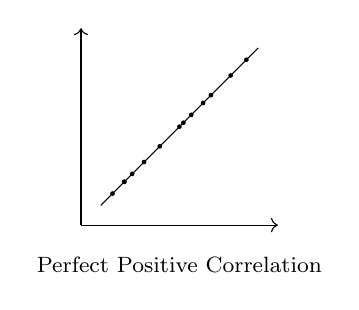
\begin{tikzpicture}[scale=0.5]
      \draw[->] (0, 0) -- (5, 0);
      \draw[->] (0, 0) -- (0, 5);
      \draw (0.5, 0.5) -- (4.5, 4.5);
      \fill (0.8, 0.8) circle (0.06);
      \fill (1.1, 1.1) circle (0.06);
      \fill (1.1, 1.1) circle (0.06);
      \fill (1.3, 1.3) circle (0.06);
      \fill (1.6, 1.6) circle (0.06);
      \fill (2.0, 2.0) circle (0.06);
      \fill (2.5, 2.5) circle (0.06);
      \fill (2.6, 2.6) circle (0.06);
      \fill (2.8, 2.8) circle (0.06);
      \fill (3.1, 3.1) circle (0.06);
      \fill (3.3, 3.3) circle (0.06);
      \fill (3.8, 3.8) circle (0.06);
      \fill (4.2, 4.2) circle (0.06);
      \node at (2.5, -1) {\footnotesize{Perfect Positive Correlation}};
    \end{tikzpicture}
    \hspace{1cm}
    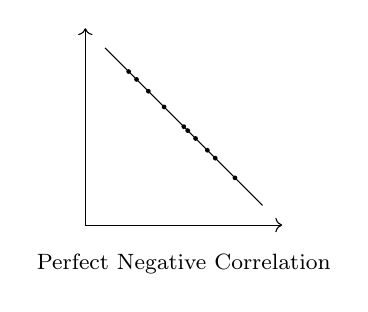
\begin{tikzpicture}[scale=0.5]
      \draw[->] (0, 0) -- (5, 0);
      \draw[->] (0, 0) -- (0, 5);
      \draw (0.5, 4.5) -- (4.5, 0.5);
      \fill (1.1, 3.9) circle (0.06);
      \fill (1.3, 3.7) circle (0.06);
      \fill (1.6, 3.4) circle (0.06);
      \fill (2.0, 3.0) circle (0.06);
      \fill (2.5, 2.5) circle (0.06);
      \fill (2.6, 2.4) circle (0.06);
      \fill (2.8, 2.2) circle (0.06);
      \fill (3.1, 1.9) circle (0.06);
      \fill (3.3, 1.7) circle (0.06);
      \fill (3.8, 1.2) circle (0.06);
      \node at (2.5, -1) {\footnotesize{Perfect Negative Correlation}};
    \end{tikzpicture}
  \end{center}
  \begin{center}
    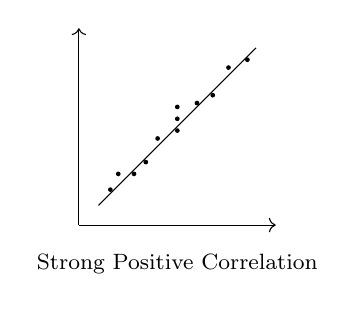
\begin{tikzpicture}[scale=0.5]
      \draw[->] (0, 0) -- (5, 0);
      \draw[->] (0, 0) -- (0, 5);
      \draw (0.5, 0.5) -- (4.5, 4.5);
      \fill (0.8, 0.9) circle (0.06);
      \fill (1.0, 1.3) circle (0.06);
      \fill (1.4, 1.3) circle (0.06);
      \fill (1.7, 1.6) circle (0.06);
      \fill (2.0, 2.2) circle (0.06);
      \fill (2.5, 2.4) circle (0.06);
      \fill (2.5, 2.7) circle (0.06);
      \fill (2.5, 3.0) circle (0.06);
      \fill (3.0, 3.1) circle (0.06);
      \fill (3.4, 3.3) circle (0.06);
      \fill (3.8, 4.0) circle (0.06);
      \fill (4.28, 4.2) circle (0.06);
      \node at (2.5, -1) {\footnotesize{Strong Positive Correlation}};
    \end{tikzpicture}
    \hspace{1cm}
    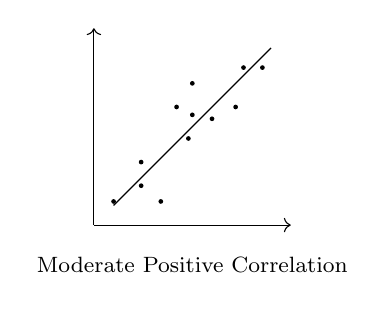
\begin{tikzpicture}[scale=0.5]
      \draw[->] (0, 0) -- (5, 0);
      \draw[->] (0, 0) -- (0, 5);
      \draw (0.5, 0.5) -- (4.5, 4.5);
      \fill (0.5, 0.6) circle (0.06);
      \fill (1.2, 1.6) circle (0.06);
      \fill (1.7, 0.6) circle (0.06);
      \fill (1.2, 1.0) circle (0.06);
      \fill (2.4, 2.2) circle (0.06);
      \fill (2.5, 2.8) circle (0.06);
      \fill (2.5, 3.6) circle (0.06);
      \fill (2.1, 3.0) circle (0.06);
      \fill (3.0, 2.7) circle (0.06);
      \fill (3.6, 3.0) circle (0.06);
      \fill (3.8, 4.0) circle (0.06);
      \fill (4.28, 4.0) circle (0.06);
      \node at (2.5, -1) {\footnotesize{Moderate Positive Correlation}};
    \end{tikzpicture}
  \end{center}
  \begin{center}
    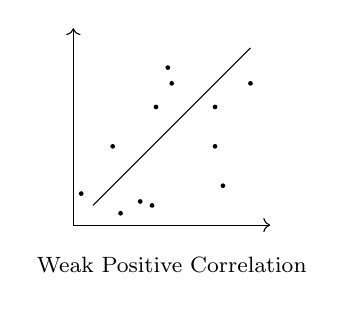
\begin{tikzpicture}[scale=0.5]
      \draw[->] (0, 0) -- (5, 0);
      \draw[->] (0, 0) -- (0, 5);
      \draw (0.5, 0.5) -- (4.5, 4.5);
      \fill (0.2, 0.8) circle (0.06);
      \fill (1.0, 2.0) circle (0.06);
      \fill (1.7, 0.6) circle (0.06);
      \fill (1.2, 0.3) circle (0.06);
      \fill (2.4, 4.0) circle (0.06);
      \fill (2.5, 3.6) circle (0.06);
      \fill (2.0, 0.5) circle (0.06);
      \fill (2.1, 3.0) circle (0.06);
      \fill (3.6, 2.0) circle (0.06);
      \fill (3.6, 3.0) circle (0.06);
      \fill (3.8, 1.0) circle (0.06);
      \fill (4.5, 3.6) circle (0.06);
      \node at (2.5, -1) {\footnotesize{Weak Positive Correlation}};
    \end{tikzpicture}
    \hspace{1cm}
    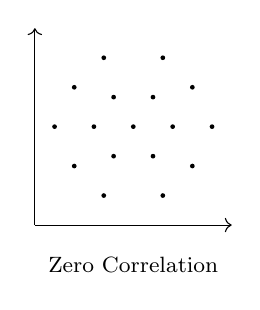
\begin{tikzpicture}[scale=0.5]
      \draw[->] (0, 0) -- (5, 0);
      \draw[->] (0, 0) -- (0, 5);
      \fill (1.75, 4.25) circle (0.06);
      \fill (3.25, 4.25) circle (0.06);
      \fill (1.0, 3.5) circle (0.06);
      \fill (4.0, 3.5) circle (0.06);
      \fill (2, 3.25) circle (0.06);
      \fill (3, 3.25) circle (0.06);
      \fill (0.5, 2.5) circle (0.06);
      \fill (1.5, 2.5) circle (0.06);
      \fill (2.5, 2.5) circle (0.06);
      \fill (3.5, 2.5) circle (0.06);
      \fill (4.5, 2.5) circle (0.06);
      \fill (1.0, 1.5) circle (0.06);
      \fill (4.0, 1.5) circle (0.06);
      \fill (2.0, 1.75) circle (0.06);
      \fill (3.0, 1.75) circle (0.06);
      \fill (1.75, 0.75) circle (0.06);
      \fill (3.25, 0.75) circle (0.06);
      \node at (2.5, -1) {\footnotesize{Zero Correlation}};
    \end{tikzpicture}
  \end{center}

  \begin{enumerate}
    \item If every single point in the scatter plot is on the line of best fit, then it's
          a perfect positive correlation. If the slope of the line of best fit is
          positive, then it's a positive correlation. If the slope of the line of best
          fit is negative, then it's a negative correlation.

    \item If the points in the scatter plot are scattered around the line of best fit
          with non-zero slope, then the closer the points are to the line of best fit,
          the stronger the correlation is.

    \item If the points in the scatter plot are scattered evenly around the whole plot
          with no obvious pattern, then there is no correlation between the two
          variables, aka zero correlation.
  \end{enumerate}

  \subsection*{Correlation Coefficient}

  Telling the correlation between two variables by looking at the scatter plot is
  not a very accurate way. To accurately measure the correlation between two sets
  of data, we need to use a coefficient that can distinguish the strength of the
  correlation.

  \begin{center}
    \begin{tikzpicture}
      \draw[->] (0, 0) -- (5, 0);
      \draw[->] (0, 0) -- (0, 5);
      \draw[dashed] (2.2, 0.0) -- (2.2, 5.0);
      \draw[dashed] (0.0, 2.2) -- (5.0, 2.2);
      \fill (0.2, 0.8) circle (0.06);
      \fill (1.0, 2.0) circle (0.06);
      \fill (1.7, 0.6) circle (0.06);
      \fill (1.2, 0.3) circle (0.06);
      \fill (2.4, 4.0) circle (0.06);
      \fill (2.5, 3.6) circle (0.06);
      \fill (2.0, 0.5) circle (0.06);
      \fill (2.1, 3.0) circle (0.06);
      \fill (3.6, 2.0) circle (0.06);
      \fill (3.6, 3.0) circle (0.06);
      \fill (3.8, 1.0) circle (0.06);
      \fill (4.5, 3.6) circle (0.06);
    \end{tikzpicture}
  \end{center}

  Let the mean value of two sets of data be $x_1, x_2, \dots, x_n$ and $y_1, y_2,
    \dots, y_n$ be $\bar{x}$ and $\bar{y}$ respectively. Draw two lines $x =
    \bar{x}$ and $y = \bar{y}$ on the scatter plot of the two sets of data,
  splitting the plot into four quadrants, as shown in the figure above. Now the
  origin of the plot is at $(\bar{x}, \bar{y})$. If a point $(x_i, y_i)$ is in
  the first or the third quadrant, then $(x_i - \bar{x})(y_i - \bar{y})$ is
  positive. As discussed in the previous section, if the correlation is positive,
  the points are scattering around the line of best fit with positive slope.
  Therefore, the points are more likely to be in the first or the third quadrant.
  That means, there are more positive value of $(x_i - \bar{x})(y_i - \bar{y})$
  than negative value, therefore the value of $\sum{(x_i - \bar{x})(y_i -
      \bar{y})}$ is positive. The higher the correlation is, the more points are in
  the first or the third quadrant, the higher the positive value of $\sum{(x_i -
      \bar{x})(y_i - \bar{y})}$ is.

  On the other hand, if a point $(x_i, y_i)$ is in the second or the fourth
  quadrant, then $(x_i - \bar{x})(y_i - \bar{y})$ is negative, which means there
  are more negative value of $(x_i - \bar{x})(y_i - \bar{y})$ than positive
  value, therefore the value of $\sum{(x_i - \bar{x})(y_i - \bar{y})}$ is
  negative. Similarly, he higher the correlation is, the lower the negative value
  of $\sum{(x_i - \bar{x})(y_i - \bar{y})}$ is.

  Hence, the value and the sign of $\sum{(x_i - \bar{x})(y_i - \bar{y})}$ can be
  used to measure the correlation between two sets of data. The value of
  $\sum{(x_i - \bar{x})(y_i - \bar{y})}$ will be affected by the measurement unit
  of the data. To make the value of $\sum{(x_i - \bar{x})(y_i - \bar{y})}$
  independent of the measurement unit, we define the correlation coefficient of
  two sets of data $x_1, x_2, \dots, x_n$ and $y_1, y_2, \dots, y_n$ as:

  \begin{cequation}
    r = \frac{\sum{(x_i - \bar{x})(y_i - \bar{y})}}{\sqrt{\sum{(x_i - \bar{x})^2}\sum{(y_i - \bar{y})^2}}}
  \end{cequation}

  The value of $r$ is always between $-1$ and $1$. If $r = 0$, then there is no
  correlation between the two sets of data. If $r > 0$, then the correlation is
  positive. If $r < 0$, then the correlation is negative. The absolute value of
  $r$ is the strength of the correlation, and is generally divided as follows:

  \begin{enumerate}
    \item $|r| = 1$: perfect correlation
    \item $0 < |r| < 0.3$: weak correlation
    \item $0.3 \leq |r| < 0.7$: moderate correlation
    \item $0.7 \leq |r| \leq 1$: strong correlation
  \end{enumerate}

  Dividing both the denominator and the numerator of the formula of $r$ by the
  number of data points $n$, then the numerator is the mean value of $(x_i -
    \bar{x})(y_i - \bar{y})$, and the denominator is the product of the standard
  deviation of $x_1, x_2, \dots, x_n$ and $y_1, y_2, \dots, y_n$. Similar to the
  standard deviation, there is an easier way to calculate the correlation
  coefficient:

  \begin{cequation}
    r = \frac{\frac{\sum{x_iy_i}}{n} - \bar{x}\bar{y}}{\sqrt{(\frac{\sum{x_i^2}}{n} - \bar{x}^2)(\frac{\sum{y_i^2}}{n} - \bar{y}^2)}}
  \end{cequation}

  \subsection{Practice 10}

  \begin{enumerate}
    \item The table below shows the height (in $cm$) and weight (in $kg$) of 15
          10-year-old children:
          \begin{center}
            \begin{tabular}{|c|c|}
              \hline
              Height & Weight \\
              \hline
              126    & 41     \\
              130    & 42     \\
              110    & 38     \\
              123    & 36     \\
              118    & 33     \\
              130    & 45     \\
              127    & 34     \\
              124    & 35     \\
              116    & 30     \\
              112    & 32     \\
              113    & 31     \\
              121    & 40     \\
              115    & 34     \\
              120    & 35     \\
              118    & 33     \\
              \hline
            \end{tabular}
          \end{center}
          Calculate the correlation coefficient of the height and the weight of the 15 children, and determine on the strength of the correlation.

    \item In order to study the relationship between the systolic blood pressure (in
          $\mathit{mmHg}$) and the age (in $year$) of human, a medical school collected
          the data of 13 male patients:
          \begin{center}
            \begin{tabular}{|c|c|}
              \hline
              Age & Systolic Blood Pressure \\
              \hline
              51  & 130                     \\
              22  & 141                     \\
              23  & 124                     \\
              31  & 126                     \\
              33  & 117                     \\
              49  & 135                     \\
              58  & 143                     \\
              53  & 138                     \\
              44  & 132                     \\
              55  & 143                     \\
              42  & 133                     \\
              45  & 115                     \\
              25  & 147                     \\
              \hline
            \end{tabular}
          \end{center}
  \end{enumerate}

  \subsection{Exercise 18.6}

  \begin{enumerate}
    \item The table below shows the value of fixed assets and total assets (in 10
          thousand dollar) of 10 enterprises of the same industry:
          \begin{center}
            \begin{tabular}{|c|c|c|}
              \hline
              No. of Enterprise & Fixed Assets & Total Assets \\
              \hline
              1                 & 200          & 638          \\
              2                 & 314          & 605          \\
              3                 & 318          & 524          \\
              4                 & 409          & 815          \\
              5                 & 415          & 913          \\
              6                 & 502          & 928          \\
              7                 & 910          & 1019         \\
              8                 & 1022         & 1219         \\
              9                 & 1210         & 1516         \\
              10                & 1225         & 1624         \\
              \hline
            \end{tabular}
          \end{center}
          \begin{enumerate}
            \item Construct a scatter diagram of the data.
            \item Calculate the mean value of fixed assets and total assets respectively.
            \item Find the correlation coefficient of the fixed assets and the total assets, and
                  determine on the strength of the correlation.
          \end{enumerate}

    \item The table shows the marks of Mathematics and Ecomoics of 15 students:
          \begin{center}
            \begin{tabular}{|c|c|}
              \hline
              Mathematics & Economics \\
              \hline
              83          & 79        \\
              50          & 61        \\
              62          & 70        \\
              90          & 86        \\
              68          & 69        \\
              61          & 68        \\
              58          & 62        \\
              62          & 80        \\
              71          & 70        \\
              63          & 74        \\
              72          & 77        \\
              54          & 54        \\
              64          & 77        \\
              48          & 50        \\
              81          & 92        \\
              \hline
            \end{tabular}
          \end{center}
          \begin{enumerate}
            \item Construct a scatter diagram of the data.
            \item Find the correlation coefficient of the marks of Mathematics and the Economics,
                  and determine on the strength of the correlation.
          \end{enumerate}

    \item The table below shows the marks of 16 students in the Chinese language minor
          test. The paper was split into two sections: Vernacular and Classical Chinese
          and their full marks were 60 and 40 respectively.
          \begin{center}
            \begin{tabular}{|c|c|}
              \hline
              Vernacular Chinese & Classical Chinese \\
              \hline
              43                 & 30                \\
              50                 & 21                \\
              38                 & 20                \\
              45                 & 19                \\
              58                 & 15                \\
              47                 & 18                \\
              32                 & 30                \\
              36                 & 28                \\
              38                 & 26                \\
              51                 & 30                \\
              44                 & 29                \\
              28                 & 29                \\
              49                 & 22                \\
              42                 & 32                \\
              46                 & 33                \\
              35                 & 25                \\
              \hline
            \end{tabular}
          \end{center}
          \begin{enumerate}
            \item Construct a scatter diagram of the data.
            \item Find the correlation coefficient of the marks of Vernacular Chinese and the
                  Classical Chinese, and determine on the strength of the correlation.
          \end{enumerate}

    \item Below shows the the service costs and values of properties sold by a property
          broker in 5 trades:
          \begin{center}
            \begin{tabular}{|c|c|}
              \hline
              Service Costs (in \$100) & Value of Prop. (in \$10k) \\
              \hline
              16.5                     & 3.9                       \\
              17.4                     & 4.2                       \\
              16.8                     & 4.1                       \\
              17.9                     & 4.5                       \\
              18.4                     & 4.8                       \\
              \hline
            \end{tabular}
          \end{center}
          Find the correlation coefficient of the service costs and the values of properties in these 5 trades, and determine on the strength of the correlation.

    \item The table below shows the degree of labor mechanization and labor productivity:
          \begin{center}
            \begin{tabular}{|c|c|}
              \hline
              Mechanization Degree (\%) & Productivity (\$/pax) \\
              \hline
              40                        & 800                   \\
              45                        & 880                   \\
              50                        & 1010                  \\
              55                        & 1034                  \\
              60                        & 980                   \\
              65                        & 1030                  \\
              70                        & 1077                  \\
              75                        & 1344                  \\
              80                        & 1460                  \\
              \hline
            \end{tabular}
          \end{center}
          \begin{enumerate}
            \item Construct a scatter diagram of the data.
            \item Find the correlation coefficient of the degree of labor mechanization and the
                  labor productivity, and determine on the strength of the correlation.
          \end{enumerate}

    \item Below are the sales (in million) and the net profit rate (\%) of 10 department
          store:
          \begin{center}
            \begin{tabular}{|c|c|c|}
              \hline
              Company & Sales & Net Profit Rate \\
              \hline
              A       & 18.4  & 15.3            \\
              B       & 16.5  & 14.8            \\
              C       & 14.6  & 13.6            \\
              D       & 23.3  & 14.3            \\
              E       & 35.6  & 12.9            \\
              F       & 24.2  & 14.6            \\
              G       & 33.6  & 13.8            \\
              H       & 44.5  & 13.7            \\
              I       & 26.8  & 13.5            \\
              J       & 31.9  & 14.2            \\
              \hline
            \end{tabular}
          \end{center}
          \begin{enumerate}
            \item Construct a scatter diagram of the data.
            \item Find the correlation coefficient of the sales and the net profit rate, and
                  determine on the strength of the correlation.
          \end{enumerate}

  \end{enumerate}

  \section{Statistical Index}

  \subsection*{Index}

  In statistics, an index is a number that measures the changes in a figure from
  one point in time to another. There is a wide range of applications of an
  index, such as the price index which represents the changes in prices, the
  production index which represents the changes in production, and the wage index
  which represents the changes in salaries and wages. There are also other
  indices such as the living index, foreign exchange index, population index,
  stock market index, etc.

  The index is a kind of relative number. The standard period that is used for
  comparison when calculating the index is called the base period. As the case
  may be, the base period can be a year or a month. The index of the base period
  is usually a number that is easier to be remembered and compared, such as 100,
  500, or 1000, and the chosen number must be able to represent the changes in
  the figure. We will use 100 as our base period index. The period that is used
  for comparison to the base period is called the current period. Let $Q_0$ be
  the base period index and $Q_1$ be the current period index. The index of the
  current period is calculated by the following formula:

  \begin{cequation}
    I = \frac{Q_1}{Q_0} \times 100
  \end{cequation}

  \noindent where 100 is the base period index.

  \subsection*{Price Relative}

  The price relative is a simple index that compares the prices of products in
  different periods. Let $P_0$ be the price of a product in the base period and
  $P_1$ be the price of the same product in the current period. The price
  relative of the current period is calculated by the following formula:

  \begin{cequation}
    I = \frac{P_1}{P_0} \times 100
  \end{cequation}

  \subsection{Practice 11}

  The table below shows the net profits (in million) of a company from 2010 to
  2014. Use the year 2010 as the base period and calculate the index of the net
  profit of the company in each year.
  \begin{center}
    \begin{tabular}{|c|c|c|c|c|c|}
      \hline
      Year       & 2010 & 2011 & 2012  & 2013  & 2014 \\
      \hline
      Net Profit & 700  & 621  & 584.1 & 720.5 & 800  \\
      \hline
    \end{tabular}
  \end{center}

  \subsection*{Exercise 18.7a}

  \begin{enumerate}
    \item The prices of white sugar in 2011, 2012, and 2013 are \$2.10, \$2.30, and
          \$2.50 respectively. Use the year 2011 and 2012 as the base period and
          calculate the price relative of the year 2013.

    \item The prices of a food product in 2011, 2013, and 2015 are \$3.40, \$3.75, and
          \$3.90 respectively. Use the year 2011 as the base period and calculate the
          price relative of the year 2013 and 2015.

    \item The number of new students of a school from 2011 to 2015 are as follows:
          \begin{center}
            \begin{tabular}{|c|c|c|c|c|c|}
              \hline
              Year      & 2011 & 2012 & 2013 & 2014 & 2015 \\
              \hline
              New Stud. & 182  & 150  & 120  & 104  & 94   \\
              \hline
            \end{tabular}
          \end{center}
          Use the year 2011 as the base period and calculate the index of the number of new students in each year.

    \item The table below shows the price of terraced houses (in \$10k) of a place in
          from 2019 to 2014:
          \begin{center}
            \begin{tabular}{|c|c|c|c|c|c|}
              \hline
              Year  & 2010 & 2011 & 2012 & 2013 & 2014 \\
              \hline
              Price & 32.0 & 35.5 & 43.4 & 51.0 & 60.0 \\
              \hline
            \end{tabular}
          \end{center}
          Use the year 2010 as the base period and calculate the index of the price of terraced houses in each year.

    \item The table below shows the price relative of three products $A$, $B$, and $C$
          when using different years as the base period and the current period:
          \begin{center}
            \begin{tabular}{|c|c|c|c|c|}
              \hline
              Current Period & Base Period & $A$ & $B$ & $C$ \\
              \hline
              2010           & 2005        & 160 & $x$ & 170 \\
              2015           & 2005        & 140 & 190 & $y$ \\
              2015           & 2010        & $z$ & 210 & 150 \\
              \hline
            \end{tabular}
          \end{center}
          Find the value of $x$, $y$, and $z$.

  \end{enumerate}

  \subsection*{Composite Index}

  The composite index is the mean value of indices of different figures. Since
  the importance of each figure might be different, the weight of each index is
  used to represent the importance of each figure, and the acquired weighted mean
  is called the composite index.

  Let the simple index of $n$ figures of the same base period and the same
  current period be $x_1, x_2, \ldots, x_n$, and their respective weights be
  $w_1, w_2, \ldots, w_n$. The composite index is calculated by the following
  formula:

  \makeatletter
  \setbool{@fleqn}{false}
  \makeatother
  \begin{flalign*}
    \bar{I} & = \frac{w_1x_1 + w_2x_2 + \cdots + w_nx_n}{w_1 + w_2 + \cdots + w_n} \\
            & = \frac{\sum{w_ix_i}}{\sum{w_i}}
  \end{flalign*}
  \makeatletter
  \setbool{@fleqn}{true}
  \makeatother

  If the study object is some product, where $x_i$ is the price relative to the
  $i^{th}$ product, then its weighted mean is called the price index. If the
  study object is the daily living expenses, then its weighted mean is called the
  living consumption index.

  \subsection*{Practice 12}

  The table below shows the prices and weights of sneakers of three brands in
  2012 and 2015:
  \begin{center}
    \begin{tabular}{|c|c|c|c|}
      \hline
      \multirow{2}{*}{Sneakers} & \multicolumn{2}{c|}{Unit Price} & \multirow{2}{*}{Weight}     \\
      \cline{2-3}
                                & 2012                            & 2015                    &   \\
      \hline
      A                         & 230                             & 233                     & 5 \\
      B                         & 225                             & 228                     & 3 \\
      C                         & 215                             & 221                     & 2 \\
      \hline
    \end{tabular}
  \end{center}
  \begin{enumerate}
    \item Use the year 2012 as the base period and calculate the price relative of each
          brand in 2015.
    \item Use the year 2012 as the base period and calculate the price index of sneakers
          in 2015.
  \end{enumerate}

  \subsection*{Exercise 18.7b}

  \begin{enumerate}
    \item Using 2012 as the base period, the price relatives of foods, gases and clothes
          in 2014 are 111, 105, and 106 respectively, and their weights are 5, 1, and 2
          respectively. Calculate the composite index of the three comsumer items in
          2014.

    \item The table below shows the price of each primary food in 2015 (with 2005 as the
          base period). Find the price index in 2015.
          \begin{center}
            \begin{tabular}{|c|c|c|}
              \hline
              Food        & Price Relative & Weight \\
              \hline
              Meat        & 130            & 15     \\
              Fish        & 150            & 14     \\
              Vegetable   & 200            & 10     \\
              Rice        & 110            & 20     \\
              Cooking Oil & 120            & 8      \\
              Beverage    & 150            & 7      \\
              Fruit       & 160            & 6      \\
              \hline
            \end{tabular}
          \end{center}

    \item The weight and unit price of 3 kind of materials bought by a factory are as
          follows:
          \begin{center}
            \begin{tabular}{|c|c|c|c|}
              \hline
              \multirow{2}{*}{Material} & \multirow{2}{*}{Weight (ton)} & \multicolumn{2}{c|}{Unit Price (\$)}        \\
              \cline{3-4}
                                        &                               & 2010                                 & 2014 \\
              \hline
              A                         & 20                            & 0.62                                 & 0.71 \\
              B                         & 50                            & 2.05                                 & 2.09 \\
              C                         & 60                            & 0.80                                 & 0.85 \\
              \hline
            \end{tabular}
          \end{center}
          Using 2010 as the base period, 2014 as the current period,
          \begin{enumerate}
            \item Find the composite index of the unit prices of the three materials without
                  considering the weights (i.e. the weights are all 1).
            \item Using the weight of each material as the weight, find the composite index of
                  the unit prices of the three materials.
          \end{enumerate}

    \item The table below shows three indices and their weights. If their composite index
          is 103, find the value of $x$.
          \begin{center}
            \begin{tabular}{|c|c|c|c|}
              \hline
              Index  & 90  & 11$x$ & 120 \\
              \hline
              Weight & $x$ & 4     & 6   \\
              \hline
            \end{tabular}
          \end{center}

    \item The table below shows the price relative and weight of three products with 2013
          as the base period and 2015 as the current period. Given that the price of item
          $A$ in 2013 and 2015 are $\$20$ and $\$25$ respectively, the price of item $B$
          is twice the price of item $A$.
          \begin{center}
            \begin{tabular}{|c|c|c|}
              \hline
              Item & Price Relative & Weight \\
              \hline
              A    & $r$            & 2      \\
              B    & $t$            & 1      \\
              C    & 120            & 3      \\
              \hline
            \end{tabular}
          \end{center}
          \begin{enumerate}
            \item Find the value of $r$ adn $t$.
            \item Using 2013 as the base period, find the price index in 2015.
          \end{enumerate}

    \item The table below shows the price relative and weight of 5 products with 2012 as
          the base period and 2014 as the current period:
          \begin{center}
            \begin{tabular}{|c|c|c|}
              \hline
              Item & Price Relative & Weight \\
              \hline
              A    & 125            & 2      \\
              B    & 120            & 3$x$   \\
              C    & 110            & 2      \\
              D    & 130            & $x$    \\
              E    & 115            & 2      \\
              \hline
            \end{tabular}
          \end{center}
          Given that the price index in 2014 is 120,
          \begin{enumerate}
            \item Find the value of $x$.
            \item Assume that the price of item $A$ in 2014 is RM30, find the price of the item
                  in 2012.
          \end{enumerate}

    \item The table below shows the price, price relative and weight of 4 products in
          2012 and 2014:
          \begin{center}
            \begin{tabular}{|c|c|c|c|c|}
              \hline
              \multirow{2}{*}{Item} & \multicolumn{2}{c|}{Price (\$)} & \multirow{2}{*}{Price Relative} & \multirow{2}{*}{Weight}     \\
              \cline{2-3}
                                    & 2012                            & 2014                            &                         &   \\
              \hline
              A                     & 12                              & $y$                             & 150                     & 1 \\
              B                     & $x$                             & 24                              & 120                     & 2 \\
              C                     & 14                              & 28                              & $z$                     & 3 \\
              D                     & 10                              & 13                              & 130                     & 4 \\
              \hline
            \end{tabular}
          \end{center}
          where the base period of the price relative is 2012, and the current period is 2014.
          \begin{enumerate}
            \item Find the value of $x$, $y$ and $z$.
            \item Using 2012 as the base period, find the price index in 2014.
          \end{enumerate}

    \item The table below shows the price of two products in 2005 and 2015:
          \begin{center}
            \begin{tabular}{|c|c|c|c|}
              \hline
              \multirow{2}{*}{Item} & \multicolumn{2}{c|}{Price (\$)} & \multirow{2}{*}{Price Relative}     \\
              \cline{2-3}
                                    & 2005                            & 2015                            &   \\
              \hline
              A                     & 30                              & $x$                             & 2 \\
              B                     & 50                              & $x+10$                          & 3 \\
              \hline
            \end{tabular}
          \end{center}

  \end{enumerate}

  \section{Revision Exercise 18}

  \begin{enumerate}
    \item The length of 60 cotten fibers (in $mm$) in a laboratory are as follows:
          \begin{flalign*}
            82  & \quad 202 \quad 352 \quad 321 \quad 25 \quad 293 \quad 293 \quad 86   & \\
            28  & \quad 206 \quad 323 \quad 355 \quad 357 \quad 33 \quad 325 \quad 113  & \\
            233 & \quad 294 \quad 50 \quad 296 \quad 115 \quad 236 \quad 357 \quad 326  & \\
            52  & \quad 301 \quad 140 \quad 328 \quad 238 \quad 358 \quad 58 \quad 255  & \\
            143 & \quad 360 \quad 340 \quad 302 \quad 370 \quad 343 \quad 260 \quad 303 & \\
            59  & \quad 146 \quad 60 \quad 263 \quad 170 \quad 175 \quad 348 \quad 305  & \\
            380 & \quad 346 \quad 61 \quad 305 \quad 264 \quad 383 \quad 62 \quad 306   & \\
            195 & \quad 350 \quad 265 \quad 385
          \end{flalign*}
          \begin{enumerate}
            \item Use $21mm$ as the lower limit and $40mm$ as the class range, construct a
                  frequency distribution table.
            \item Construct a histogram and a frequency polygon.
            \item Construct a cumulative frequency table and a cumulative frequency polygon.
            \item Using the cumulative frequency polygon, find the percentage of fibers whose
                  length is greater than $150mm$.
            \item Find the interquartile range.
          \end{enumerate}

    \item Find the mean, median, range, quartile deviation, and mean deviation of the
          data $8, 10, 9, 12, 4, 4, 2$.

    \item The weight (in $kg$) if 16 babies are as follows:
          \begin{flalign*}
            8 & \quad 9 \quad 10 \quad 9 \quad 8 \quad 7 \quad 9 \quad 10 \\
            9 & \quad 8 \quad 8 \quad 9 \quad 10 \quad 9 \quad 8 \quad 7
          \end{flalign*}
          Find the mean, meidan, mode, range, quartile deviation, mean deviation, and standard deviation of their weights.

    \item The table below shows the score distribution of business study minor test of
          senior 3 students in a high school:
          \begin{center}
            \begin{tabular}{|c|c|c|}
              \hline
              Marks & No. of Students \\
              \hline
              0-9   & 7               \\
              10-19 & 21              \\
              20-29 & 32              \\
              30-39 & 27              \\
              40-49 & 13              \\
              \hline
            \end{tabular}
          \end{center}
          \begin{enumerate}
            \item Construct a cumulative frequency distribution table.
            \item Construct a cumulative frequency polygon.
            \item Find the median and the interquartile range from the cumulative frequency
                  polygon.
            \item Find the percentage of students who scored higher or equal to 45 marks.
            \item Assume that the passing score is 15 marks. Find the percentage of students who
                  failed the test.
          \end{enumerate}

    \item The burning time (in $s$) of 10 rocket boosters are as follows: \makeatletter
          \setbool{@fleqn}{false} \makeatother
          \begin{flalign*}
            50.7 & \quad 54.9 \quad 54.3 \quad 44.8 \quad 42.2 \\
            69.0 & \quad 55.4 \quad 66.1 \quad 48.1 \quad 34.5
          \end{flalign*}
          \makeatletter
          \setbool{@fleqn}{true}
          \makeatother

          Find the range, variance and standard deviation of the burning time.

    \item The table below shows the scores of 30 rounds of game scored by someone:
          \begin{center}
            \begin{tabular}{|c|c|c|c|c|c|}
              \hline
              Score & 0 & 1 & 2 & 3     & 4 \\
              \hline
              Times & 5 & 3 & 4 & $x+1$ & 7 \\
              \hline
            \end{tabular}
          \end{center}
          Find:
          \begin{enumerate}
            \item The value of $x$.
            \item The mean and standard deviation of the scores.
          \end{enumerate}

    \item The table below shows the distribution of scores of a minor test of students in
          a class:
          \begin{center}
            \begin{tabular}{|c|c|}
              \hline
              Score            & No. of Students \\
              \hline
              $0 < x \leq 5$   & 8               \\
              $5 < x \leq 10$  & 1               \\
              $10 < x \leq 15$ & 9               \\
              $15 < x \leq 20$ & 7               \\
              $20 < x \leq 25$ & 11              \\
              $25 < x \leq 30$ & 4               \\
              \hline
            \end{tabular}
          \end{center}
          Find:
          \begin{enumerate}
            \item Range
            \item Median
            \item Mode
          \end{enumerate}

    \item Below are the distribution of scores of business study exam of 40 students in a
          class:
          \begin{center}
            \begin{tabular}{|c|c|}
              \hline
              Score   & No. of Students \\
              \hline
              46 - 54 & 4               \\
              54 - 62 & 9               \\
              62 - 70 & 10              \\
              70 - 78 & 8               \\
              78 - 86 & 6               \\
              86 - 94 & 3               \\
              \hline
            \end{tabular}
          \end{center}
          Find:
          \begin{enumerate}
            \item Mean
            \item Median
            \item Mode
            \item Variance
          \end{enumerate}

    \item The table below shows the frequency distribution of the life of 500 light
          bulbs:
          \begin{center}
            \begin{tabular}{|c|c|}
              \hline
              Life (in $hr$) & No. of Bulbs \\
              \hline
              800 - 850      & 35           \\
              850 - 900      & 127          \\
              900 - 950      & 185          \\
              950 - 1000     & 103          \\
              1000 - 1050    & 42           \\
              1050 - 1100    & 8            \\
              \hline
            \end{tabular}
          \end{center}
          Find:
          \begin{enumerate}
            \item The mean and standard deviation of the life of the light bulbs.
            \item Mean deviation.
            \item Median.
            \item Quartile deviation.
          \end{enumerate}

    \item Assume that the mean value of data $2, x+1, 5, 2x+1, 8, 2x-3$ is 4,
          \begin{enumerate}
            \item Find the value of $x$.
            \item With that, find the standard deviation of the data.
          \end{enumerate}

    \item The mean and mode of a set of data $2, 5, 3, 11, 9, 2, 11, p, q$ are 6 and 3
          respectively, $p > q$. Find
          \begin{enumerate}
            \item The value of $p$ and $q$
            \item Median
            \item Standard deviation
          \end{enumerate}

    \item Given that the mean value of $x, x+1, 2x-3, 5, y, 8$ is 6. After eliminating
          $y$, the mean value of the remaining data is $3.8$.
          \begin{enumerate}
            \item Find the value of $x$ and $y$.
            \item With that, find the variance of the original 6 data.
          \end{enumerate}

    \item Given the sum of the square of 10 numbers is 400, and their mean value is 5. If
          a number 8 is eliminated from the data set, find the mean value and variance of
          the remaining data.

    \item There are two female chorus groups $A$ and $B$, each of which has 5 members.
          Their heights (in $cm$) are as follows:
          \begin{center}
            \begin{tabular}{|c|c|}
              \hline
              Group A & 170 \quad 162 \quad 159 \quad 160 \quad 155 \\
              \hline
              Group B & 180 \quad 165 \quad 150 \quad 154 \quad 160 \\
              \hline
            \end{tabular}
          \end{center}
          \begin{enumerate}
            \item Find the mean and standard deviation of the heights of the members of the two
                  groups.
            \item Which group has a lower height variance?
          \end{enumerate}

    \item The table below shows scores of maths exam of three classes:
          \begin{center}
            \begin{tabular}{|c|c|c|c|}
              \hline
              Class & Avg. Marks & Std. Deviation & No. of Stud. \\
              \hline
              A     & 36.8       & 5.2            & 32           \\
              B     & 30.3       & 12.4           & 36           \\
              C     & 38.8       & 10.3           & 32           \\
              \hline
            \end{tabular}
          \end{center}
          \begin{enumerate}
            \item In between class $A$, $B$ and $C$, which class has the most consistent
                  performance? Why?
            \item Find the average marks and standard deviation of these three classes combined.
          \end{enumerate}

    \item The score given by six judges to a gymnast are as follows: \makeatletter
          \setbool{@fleqn}{false} \makeatother
          \begin{flalign*}
            7 \quad 5 \quad 9 \quad 7 \quad 8 \quad 6
          \end{flalign*}
          \makeatletter
          \setbool{@fleqn}{true}
          \makeatother
          Find the following of the gymnast:
          \begin{enumerate}
            \item Mean
            \item Standard deviation
            \item Correlation Coefficient
          \end{enumerate}

    \item In an IQ test, the average score of 10 students is 114, and the scores of 9 of
          them are as follows: \makeatletter \setbool{@fleqn}{false} \makeatother
          \begin{flalign*}
            101 & \quad 125 \quad 118 \quad 118 \quad 128 \quad 106 \\
            115 & \quad 99 \quad 118 \quad 109
          \end{flalign*}
          \makeatletter
          \setbool{@fleqn}{true}
          \makeatother
          Find:
          \begin{enumerate}
            \item The IQ of the 10th student.
            \item The correlation coefficient of the IQ of the 10 students.
          \end{enumerate}

    \item Given that the data of the weight of two groups of girls (in $kg$) are as
          follows:
          \begin{center}
            \begin{tabular}{|c|c|c|}
              \hline
                          & Mean  & Std. Dev. \\
              \hline
              1 years old & 10.90 & 1.24      \\
              5 years old & 19.00 & 2.11      \\
              \hline
            \end{tabular}
          \end{center}
          Compare the strength of correlation of the weight of these girls.

    \item The prodution output and production cost of a factory in the first half of this
          year are as follows:
          \begin{center}
            \begin{tabular}{|c|c|c|c|c|c|c|}
              \hline
              Month                  & 1 & 2  & 3 & 4  & 5  & 6  \\
              \hline
              Output (in $1k\ tons$) & 2 & 3  & 1 & 4  & 3  & 5  \\
              Cost (in $\$1k$)       & 9 & 11 & 7 & 13 & 11 & 15 \\
              \hline
            \end{tabular}
          \end{center}

    \item The marks of Chinese exam and Maths exam of 16 senior students in a school are
          as follows:
          \begin{center}
            \begin{tabular}{|c|c|}
              \hline
              Chinese & Maths \\
              \hline
              82      & 59    \\
              79      & 63    \\
              76      & 99    \\
              63      & 67    \\
              56      & 61    \\
              67      & 82    \\
              69      & 82    \\
              81      & 77    \\
              77      & 75    \\
              73      & 74    \\
              58      & 67    \\
              64      & 79    \\
              68      & 75    \\
              72      & 65    \\
              75      & 64    \\
              80      & 66    \\
              83      & 68    \\
              \hline
            \end{tabular}
          \end{center}
          \begin{enumerate}
            \item Construct a scatter diagram of the data.
            \item Find the correlation coefficient of the two exams, and determine the strength
                  of correlation.
          \end{enumerate}

    \item The table below shows the prices of a product (in \$) in 2005, 2010, and 2015:
          \begin{center}
            \begin{tabular}{|c|c|c|c|}
              \hline
              Year  & 2005 & 2010 & 2015 \\
              \hline
              Price & 4    & 6    & $x$  \\
              \hline
            \end{tabular}
          \end{center}
          \begin{enumerate}
            \item Assume that the percentage of price increase from 2005 to 2010 is the same as
                  that from 2010 to 2015, find the value of $x$.
            \item Find the price relative in 2015 with respect to 2005.
          \end{enumerate}

    \item The price data of primary food of a city with 2013 as base period and 2014 as
          current period are as follows:
          \begin{center}
            \begin{tabular}{|c|c|c|}
              \hline
              Food                   & Price Relative & Weight \\
              \hline
              Meat                   & 105            & 8      \\
              Fish                   & 111            & 7      \\
              Vegetables             & 98             & 5      \\
              Rice        \& Noodles & 103            & 10     \\
              Cooking Oil            & 100            & 3      \\
              Beverage               & 107            & 2      \\
              Fruits                 & 99             & 2      \\
              \hline
            \end{tabular}
          \end{center}
          Find the price index in 2014.

    \item The price relative of daily expenses of people in a place with repsect to last
          year and their relative consumption are as follows:
          \begin{center}
            \begin{tabular}{|c|c|c|}
              \hline
              Daily Expenses & Price Relative & Consumption Relative \\
              \hline
              Clothing       & 120            & 23                   \\
              Food           & 117            & 40                   \\
              Housing        & 132            & 19                   \\
              Transportation & 130            & 18                   \\
              \hline
            \end{tabular}
          \end{center}
          Using the relative consumption as weight, find the composite price index of daily expenses.

    \item The table below shows the spending of a company in 4 different projects in 3
          consecutive years:
          \begin{center}
            \begin{tabular}{|c|c|c|c|c|c|}
              \hline
              \multirow{2}{*}{Project} & \multicolumn{3}{c|}{Year} & \multirow{2}{*}{A} & \multirow{2}{*}{B}             \\
              \cline{2-4}
                                       & 2012                      & 2013               & 2014               &     &     \\
              \hline
              Salaries                 & $x$                       & 20,000             & 30,000             & 150 & $P$ \\
              Stationery               & 5,000                     & $y$                & 7,000              & 120 & 140 \\
              Repair                   & 4,000                     & 5000               & $z$                & 125 & 150 \\
              Miscellaneous            & 8,000                     & $Q$                & 15,000             & $R$ & $R$ \\
              \hline
            \end{tabular}
          \end{center}
          Given that $A$ is the index where 2012 is the base period and 2013 is the current period; $B$ is the index where 2012 is the base period and 2014 is the current period. Find the value of $x$, $y$, $z$, $P$, $Q$, and $R$.

  \end{enumerate}

  \chapter{Permutations and Combinations}

  Permutations and combinations are the foundation of probability and statistics.
  In our daily life, we often need to calculate the number of ways of completing
  a task. These calculations are based on two basic principles: addition
  principle and multiplication principle.

  \section{Addition and Multiplication Principles}

  \begin{theorem}{Addition Principle}

    If there are $n$ methods of doing a task, the first method can be done in $m_1$
    ways, the second method can be done in $m_2$ ways, $\cdots$, the $n$th methods
    can be done in $m_n$ ways, and they are mutually exclusive, which means he task
    can be done in whatever way using whatever method, then the total number of
    ways of doing the task is
    \begin{cequation}
      m_1 + m_2 + \cdots + m_n
    \end{cequation}
  \end{theorem}

  \begin{theorem}{Multiplication Principle}

    If there are $n$ steps in doing a task, the first step can be done in $m_1$
    ways, the second step can be done in $m_2$ ways, $\cdots$, the $n$th steps can
    be done in $m_n$ ways, then the total number of ways of doing the task is
    \begin{cequation}
      m_1 \times m_2 \times \cdots \times m_n
    \end{cequation}
  \end{theorem}

  \subsection{Practice 1}
  \begin{enumerate}
    \item There are 2 Math reference books, 3 novels, and 4 storybooks of idioms. Xiao
          Hua wants to choose one book from each category. How many ways can he choose?
    \item Travelling from $A$ to $B$ can be done by bus or train. There are 4 buses and 3
          trains. How many ways are there to travel from $A$ to $B$?
  \end{enumerate}

  \subsection{Practice 19.1}
  \begin{enumerate}
    \item During the eve of a festival, there are 3 trains, 4 buses, and 4 trains from
          Johor Bahru to Pinang. How many ways are there to travel from Johor Bahru to
          Pinang during the day?

    \item One has 5 shirts and 6 pants, how many ways can he dress up?

    \item There are 4 airlines $A$, $B$, $C$, and $D$ that provide flights from Kuala
          Lumpur to Bangkok: $A$ provdies 3 flights per day, $B$ provides 2 flights per
          day, $C$ and $D$ provides 1 flight per day. How many choices are there to
          travel from Kuala Lumpur to Bangkok?

    \item How many set meal combinations are there if there are 6 type of main dishes, 5
          type of drinks, and 2 type of desserts?

    \item There are 4 doors in a classroom, student $A$ and student $B$ can enter the
          classroom through any door. How many ways are there for student $A$ and student
          $B$ to enter the classroom?

    \item A friendly match is held between 2 ping pong teams, each team has to send 3
          players, and each player has to play games with all the other players on the
          other team. How many games have to be played?

    \item Matching 8 clothes of different colors with 5 different skirts, how many ways
          are there to dress up? If the above dresses are paired with 4 pairs of shoes of
          different colors, how many ways are there to dress up?

  \end{enumerate}

  \section{Permutations and Permutation Formula}

  \subsection*{Practice 2}

  How many ways are there to arrange the numbers 1, 2, 3, 4 into a two digit
  number with no repeated digits? \sol{}

  First step: choose one of the 4 numbers as the first digit, there are 4 ways to
  do so.

  Second step: choose one of the remaining 3 numbers as the second digit, there
  are 3 ways to do so.

  According to the multiplication principle, the total number of ways to arrange
  the numbers 1, 2, 3, 4 into a two digit number with no repeated digits is $4
    \times 3 = 12$. \\\\ If there are $n$ elements, we want to pick $r$ elements
  from them and arrange them in a sequence, how many ways are there to do so?
  This question can be treated as there are $r$ empty boxes, which means this
  requires $r$ steps to complete.

  \begin{center}
    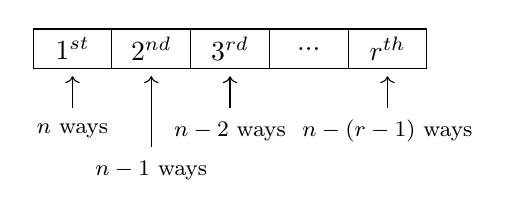
\begin{tikzpicture}
      \draw (0,0) -- (0,0.5) -- (5,0.5) -- (5,0) -- (0,0);
      \draw (1, 0) -- (1, 0.5);
      \draw (2, 0) -- (2, 0.5);
      \draw (3, 0) -- (3, 0.5);
      \draw (4, 0) -- (4, 0.5);
      \node at (0.5, 0.25) {$1^{st}$};
      \node at (1.5, 0.25) {$2^{nd}$};
      \node at (2.5, 0.25) {$3^{rd}$};
      \node at (3.5, 0.25) {$...$};
      \node at (4.5, 0.25) {$r^{th}$};
      \draw [->] (0.5, -0.5) -- (0.5, -0.1);
      \draw [->] (1.5, -1.0) -- (1.5, -0.1);
      \draw [->] (2.5, -0.5) -- (2.5, -0.1);
      \draw [->] (4.5, -0.5) -- (4.5, -0.1);
      \node at (0.5, -0.8) {\footnotesize{$n$ ways}};
      \node at (1.5, -1.3) {\footnotesize{$n-1$ ways}};
      \node at (2.5, -0.8) {\footnotesize{$n-2$ ways}};
      \node at (4.5, -0.8) {\footnotesize{$n-(r-1)$ ways}};
    \end{tikzpicture}
  \end{center}

  First step: CHhoose one element from $n$ elements and put it in the first box,
  then there are $n$ ways to do so.

  Second step: Choose one element from $n-1$ elements and put it in the second
  box, then there are $n-1$ ways to do so.

  Third step: Choose one element from $n-2$ elements and put it in the third box,
  then there are $n-2$ ways to do so.

  So on and so forth, when $r-1$ boxes are filled, the last box $r$ can only be
  filled with one of the remaining $n-(r-1)$ elements, so there are $n-(r-1)$
  ways to do so. According to the multiplication principle, the total number of
  ways to fill in $r$ boxes is
  \begin{cequation}
    n(n-1)(n-2) \cdots (n-r+1)
  \end{cequation}
  Threrefore, there are $n(n-1)(n-2) \cdots (n-r+1)$ ways to arrange $r$ elements, and this denoted as $\perm[n]{r}$, $\permtwo[n]{r}$, or $P^n_r$.
  \begin{cequation}
    \permtwo[n]{r} = n(n-1)(n-2) \cdots (n-r+1)
  \end{cequation}
  Where $r \leq n$, $n \in N$, $r = 0, 1, 2, \cdots, n$. This formula is called
  the permutation formula.

  When $r = n$, aka a full permutation, the formula becomes
  \begin{cequation}
    \permtwo[n]{n} = n(n-1)(n-2) \cdots 3 \cdot 2 \cdot 1
  \end{cequation}
  Therefore, the permutation of all $n$ elements is equal to the products of natural numbers from 1 to $n$. This is called the factorial of $n$, denoted as $n!$.
  \makeatletter
  \setbool{@fleqn}{false}
  \makeatother
  \begin{flalign*}
    n! & = \permtwo[n]{n}                       \\
       & = n(n-1)(n-2) \cdots 3 \cdot 2 \cdot 1
  \end{flalign*}
  \makeatletter
  \setbool{@fleqn}{true}
  \makeatother

  Using factorial, the permutation formula can be transform into the following:
  \begin{flalign*}
    \permtwo[n]{r} & = n(n-1)(n-2) \cdots (n-r+1)                                                                      \\
                   & = \frac{n(n-1)(n-2) \cdots (n-r+1)(n-r) \cdots 3 \cdot 2 \cdot 1}{(n-r) \cdots 3 \cdot 2 \cdot 1} \\
                   & = \frac{n!}{(n-r)!}
  \end{flalign*}

  Hence, the permutation formula can be written as
  \begin{cequation}
    \permtwo[n]{r} = \frac{n!}{(n-r)!}
  \end{cequation}

  Note: $0!$ is defined as 1 to make the formula work when $n = r$.

  \subsection{Practice 3}

  \begin{enumerate}
    \item Find the value of $\permtwo[7]{3}$ and $5!$.
    \item Calculate $\permtwo[10]{3} + \permtwo[8]{4}$.
    \item If $100(\permtwo[n]{2}) = \permtwo[2n]{3}$, find the value of $n$.
  \end{enumerate}

  \subsection{Exercise 19.2a}

  \begin{enumerate}
    \item Write down all the permutations of 3 elements in 4 elements $A$, $B$, $C$, $D$.

    \item Calculate:
          \begin{enumerate}
            \item $\permtwo[15]{4}$
            \item $\permtwo[100]{3}$
            \item $7!$
            \item $\frac{8!}{5!}$
          \end{enumerate}

    \item Calculate the following:
          \begin{enumerate}
            \item $\frac{11! - 10!}{10! - 9!}$
            \item $\frac{7! - 6! - 5!}{5!}$
            \item $\frac{13! - 12!}{{(12)}^2 10!}$
            \item $\frac{5(\permtwo[8]{3})}{2(\permtwo[6]{2})}$
            \item $\frac{\permtwo[9]{5} + \permtwo[9]{4}}{\permtwo[9]{3}}$
            \item $\frac{\permtwo{12}{12} - \permtwo{12}{11}}{\permtwo{10}{10}}$
          \end{enumerate}

    \item Simplify the following:
          \begin{enumerate}
            \item $\frac{(n+1)!}{(n-1)!}$
            \item $\frac{(20 - r)!}{(18 - r)!}$
          \end{enumerate}
  \end{enumerate}

  \section{Circular Permutations}

  \section{Full Permutations of Inexactly Distinct Elements}

  \section{Permutations with Repetition}

  \section{Combinations and Combination Formula}

  \chapter{Bionomial Theorem}

  \section{Bionomial Theorem when $n$ is a Natural Number}

  \section{General Form of Bionomial Expansion}

  \chapter{Probability}

  \section{Sample Space and Events}

  \section{Definition of Probability}

  \section{Addition Rule}

  \section{Multiplication Rule}

  \section{Mathematical Expectation}

  \section{Normal Distribution}
\end{multicols}

\end{document}